\documentclass[letterpaper, 11 pt]{article}
\usepackage[utf8]{inputenc}
\usepackage[spanish, mexico]{babel}
\usepackage{amsmath}
\usepackage{caption}
\usepackage{enumitem}
\usepackage{amsfonts}
\usepackage{apacite}
\usepackage{diagbox}
\usepackage{graphics}
\usepackage{amssymb}
\usepackage{wrapfig}
\usepackage{multicol}
\usepackage{flushend}
\usepackage{fancyhdr}
\setlength{\columnsep}{1cm}
\usepackage{appendix}
\usepackage{textcomp}
\setlength{\parskip}{7px}
\usepackage{graphicx}
\usepackage{float}
\usepackage[left=1.7cm,right=1.7cm,top=2cm,bottom=2cm]{geometry}
\usepackage{listings}
%\usepackage[breaklinks=true]{hyperref}

\begin{document}

\setlength{\unitlength}{1cm}
\thispagestyle{empty}
\begin{picture}(18,4)
\put(0,0){
\includegraphics[scale=.15]{unam.png}}
\put(14,0){
\includegraphics[scale=.19]{fac.png}}
\end{picture}

\begin{center}
\vspace*{0.2in}
{\fontsize{21}{21}\selectfont Universidad Nacional Autónoma de México}\\
\vspace*{0.2in}
{\fontsize{18}{18}\selectfont Facultad de Ciencias}\\
\vspace*{0.2in}
\begin{large}
{\fontsize{14}{14}\selectfont Laboratorio de Electromagnetismo} \\
\end{large}
\vspace*{0.2in}
\vspace*{0.2in}
\begin{Large}
\textbf{Práctica 3} \\
\textbf{Visualización de las líneas de campo y equipotenciales de una \\ región a partir del potencial mapeado.} \\
\end{Large}
\vspace{.7 cm}
Integrantes del equipo:\\
1) Alonso Barradas Luis Gustavo\\ 
2) Fragoso Alvarado Daniel\\ 
3) Rios Fematt Mildred Stephany\\ 
4) Robledo Ibarra Emiliano\\
\paragraph{}
\begin{figure}[H]
    \captionsetup{justification=centering,margin=2cm}
    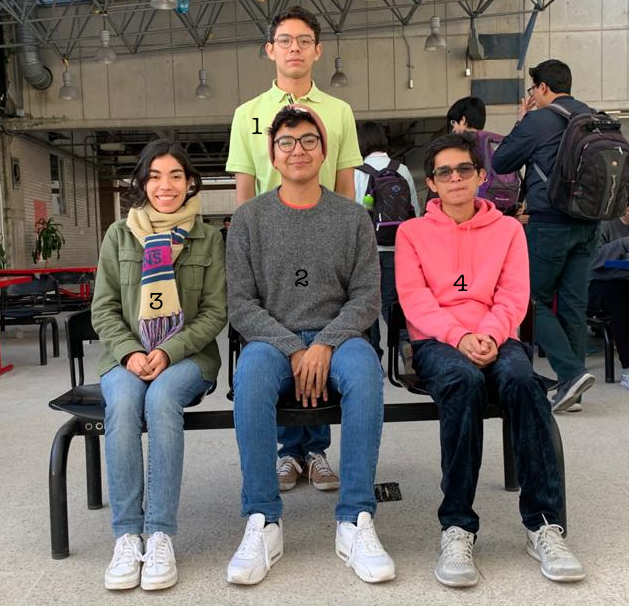
\includegraphics[scale=0.23]{uwu.jpg}
    \centering
\end{figure}
\rule{80mm}{0.1mm}\\
\begin{large}
Profesora:  Fís. Maris Sofía Flores Cruz.  \\
Ayudante: Miguel Ángel Amaya Reyes. \\
Fecha de entrega: Miercoles 11 de Marzo, 2020\\
\end{large}
\end{center}

\newpage

%------------------------------------


\begin{multicols}{2}

\section{Objetivos}
\begin{enumerate}
    \item Encontrar el valor del campo eléctrico conociendo el potencial en dos configuraciones de cargas
    \item Caracterizar un plano con las líneas equipotenciales de las distribuciones de carga y con ello encontrar las líneas de fuerza del campo eléctrico.
    \item Graficar las líneas de campo mediante las líneas que indican los niveles equipotenciales.
\end{enumerate}

\section{Introducción}
%% Antecedentes históricos %%
El \textit{campo eléctrico} --$\vec{E}$-- es una función vectorial de la posición $\vec{r}$, que es el punto donde nos interesa calcular el campo de alguna configuración de cargas eléctricas; esto quiere decir que el campo eléctrico es un campo vectorial que varia de punto a punto y se determina por la configuración de las cargas que lo generan, llamadas comúnmente fuentes. Físicamente, $\vec{ E}(\vec{r})$ es la fuerza por unidad de carga que ejercen las fuentes en algún punto $\vec{r}$ del espacio (Griffiths, 2017, p. 61).

A pesar de la definición actual que tenemos del campo eléctrico, el concepto original (introducido por Faraday a comienzos del siglo XIX) era una representación gráfica de este, sin contemplar su abstracción matemática (Resnick et. al., 2005, p. 588). Faraday planteó la visualización del campo eléctrico introduciendo el concepto de \textit{líneas de campo}, las cuales son líneas imaginarias que ayudan a visualizar cómo va variando la dirección del campo eléctrico al pasar de un punto a otro del espacio, como se muestra en la \textbf{Figura \ref{modelo}, b}. Tales líneas serán curvas (excepto en las cargas puntuales), continuas, e irán de la carga positiva a la negativa (Purcell, 1988, p. 18). 

El dibujo de una línea de campo no da directamente el valor del campo; sin embargo, las líneas de campo convergen cuando nos aproximamos a una región de campo intenso y se separan al aproximarnos a una región donde el campo es débil (Purcell, 1988, p. 17).

\begin{figure}[H]
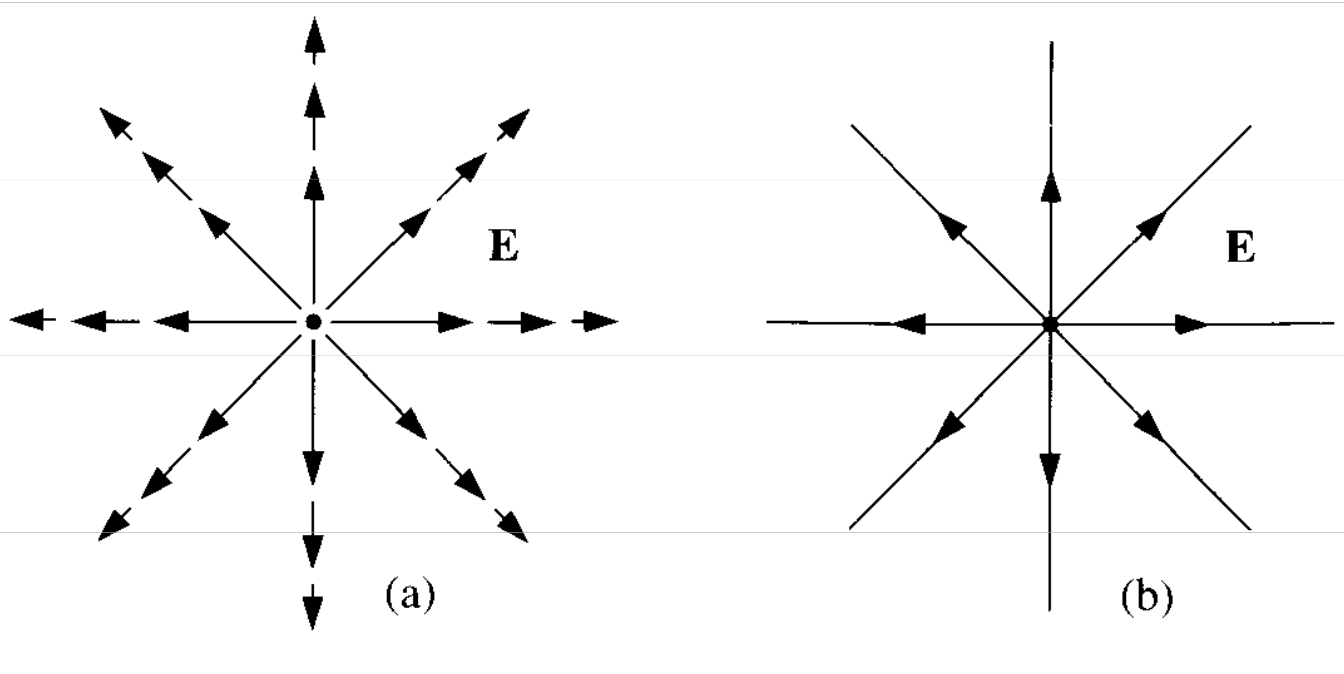
\includegraphics[scale=0.3]{Modelos.png}
\centering
\captionsetup{justification=centering,margin=0.5cm}
\caption{Esquemas gráficos del campo eléctrico de una carga puntual. \textit{Adaptado de Griffiths et.al., 2017, p. 65}}
\label{modelo}
\end{figure}

Sin embargo, no es la única forma de visualizar al campo; en la \textbf{Figura \ref{modelo}(a)} se observa una segunda forma de visualizar el campo eléctrico, donde podemos indicar el módulo y dirección de $\vec{E}$ en varios puntos dibujando pequeñas flechas a lo largo de las líneas de campo; trazando las flechas más largas donde sea más intenso y flechas más cortas en los cuales sea más débil (Purcell, 1988, p. 18). La elección de cada esquema es personal. Por términos  de simplicidad a lo largo del presente, se decidió el segundo esquema expuesto.

Pueden existir distribuciones de cargas más complejas que las cargas puntuales, en estos casos también es posible observar una representación gráfica del campo eléctrico, tal como se observa en la \textbf{Figura \ref{di}}. En esta se observa una configuración típica llamada \textit{dipolo eléctrico}, que consiste en dos cargas puntuales de signo contrario a una distancia $d$ (Griffiths, 2017, p. 66).

\begin{figure}[H]
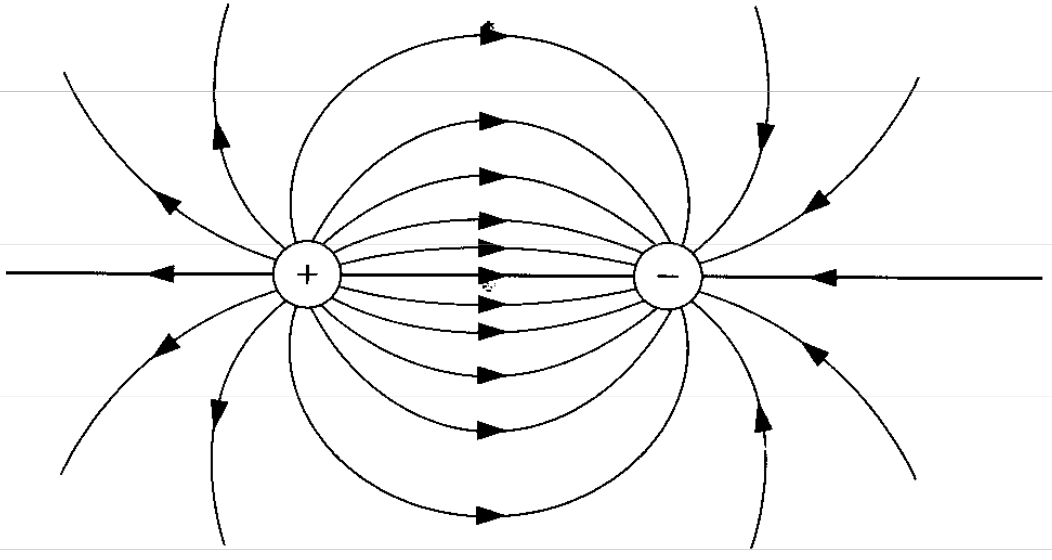
\includegraphics[scale=0.4]{dipolos.png}
\centering
\captionsetup{justification=centering,margin=0.5cm}
\caption{Esquemas gráficos del campo eléctrico en un dipolo eléctrico. \textit{Adaptado de Griffiths et.al., 2017, p. 66}}
\label{di}
\end{figure}

\paragraph{Potencial eléctrico:} bajo condiciones estáticas, si pensamos en una carga que esta inmersa en un campo eléctrico (que es un campo de fuerzas), debido a dicha interacción con el campo, la carga tendrá energía potencial. Ahora bien, el \textit{potencial eléctrico} en un punto se define como la energía potencial por unidad de carga colocada en dicho punto\footnote{El potencial eléctrico se mide en joule/coulomb o $\mathrm{J} \mathrm{C}^{-1}$, unidad que recibe el nombre de volt, abreviado $V$, en honor del científico italiano Alejandro Volta (Finn et. al., 1999, p. 480).}. Denotamos al potencial eléctrico con la letra $V$ y a la energía potencial como: $E_{p}$, de forma que la expresión que describe al potencial es (Finn et. al., 1999, p. 480):
\begin{equation}
    V = \frac{E_{p}}{q}
\end{equation}
El valor del potencial en un punto dado depende del punto que se tome como referencia inicial, por lo que, si el potencial es cero en un punto, no  necesariamente significa que la fuerza eléctrica es cero allí (Resnick et. al., 2002, p. 639 ).

Al igual que en mecánica, existe una estrecha relación entre las definiciones de campo eléctrico y el potencial eléctrico, de forma que podemos describir uno en términos del otro, como se expresa en la \textbf{Ecuación \ref{grad}} (Finn et. al., 1999, p. 480):

\begin{equation}
	\vec{E}=-\nabla V
	\label{grad}
\end{equation}

\paragraph{Superficies equipotenciales:} finalmente, de acuerdo a las distribuciones de carga, es posible encontrar superficies que tienen el mismo potencial eléctrico en todos sus puntos, es decir $V=cte=V_{0}$; estas reciben el nombre de \textit{superficies equipotenciales}. La \textbf{Figura \ref{seq}} muestra una propiedad importante de las superficies equipotenciales y el campo eléctrico: las direcciones del campo resultan perpendiculares a la superficie equipotencial en cada uno de sus puntos (Finn et. al., 1999, p. 481).

 \begin{figure}[H]
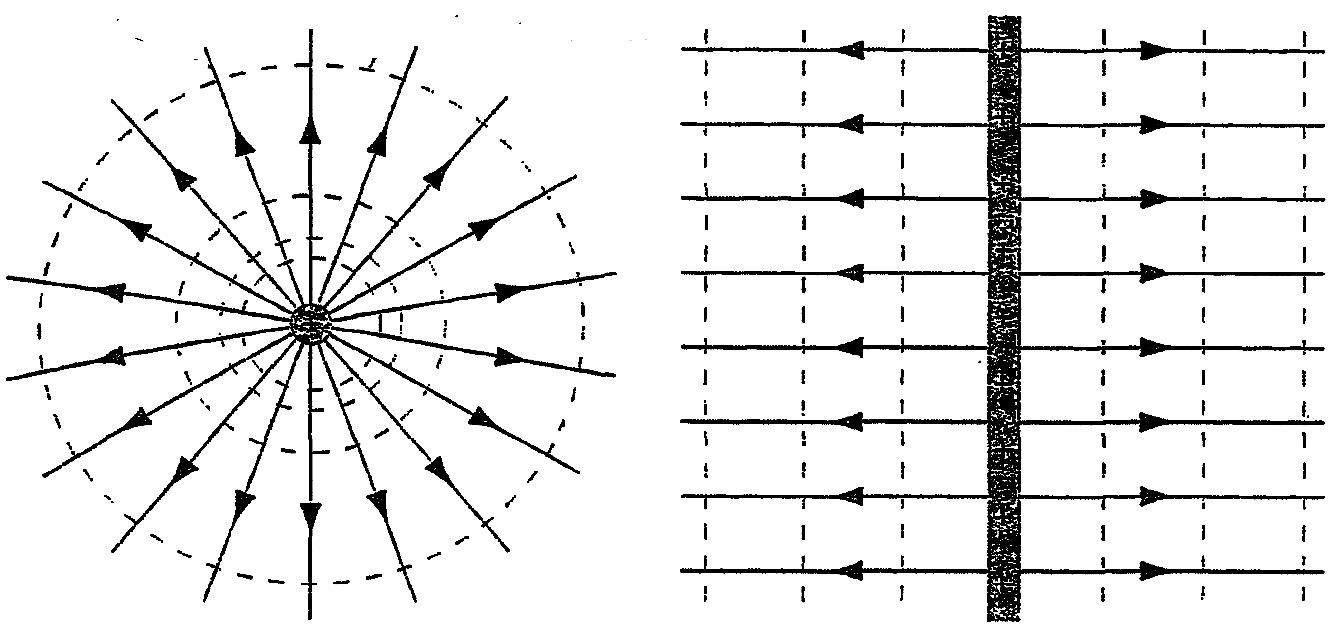
\includegraphics[scale=0.17
]{equi.jpeg}
\centering
    \captionsetup{justification=centering,margin=0.5cm}
\caption{Líneas del campo eléctrico (líneas gruesas) y superficies equipotenciales (líneas punteadas). A la izquierda una carga puntual positiva, y a la derecha una hoja infinita de carga positiva, vista a lo largo de su borde. \textit{Adaptado de Resnick et.al., 2002, p. 649}}
\label{seq}
\end{figure}

%%%%%%%%%%%
\section{Desarrollo experimental}
Para esta práctica se utilizaron los siguientes materiales:

%%% Lista de Materiales %%%
\setlist{nolistsep}
\begin{itemize}
    \item Fuente de voltaje. ($\pm 1.0\%$)
    \item Multímetro Digital. (para DC $\pm 0.8\%$)
    \item Dos hojas con figuras conductoras. (arreglo lineal y de placas)
    \item Cables conductores y caimanes.
    \item Soporte de las hojas.
\end{itemize}{}



\begin{figure}[H]
    \captionsetup{justification=centering,margin=0.5cm}
    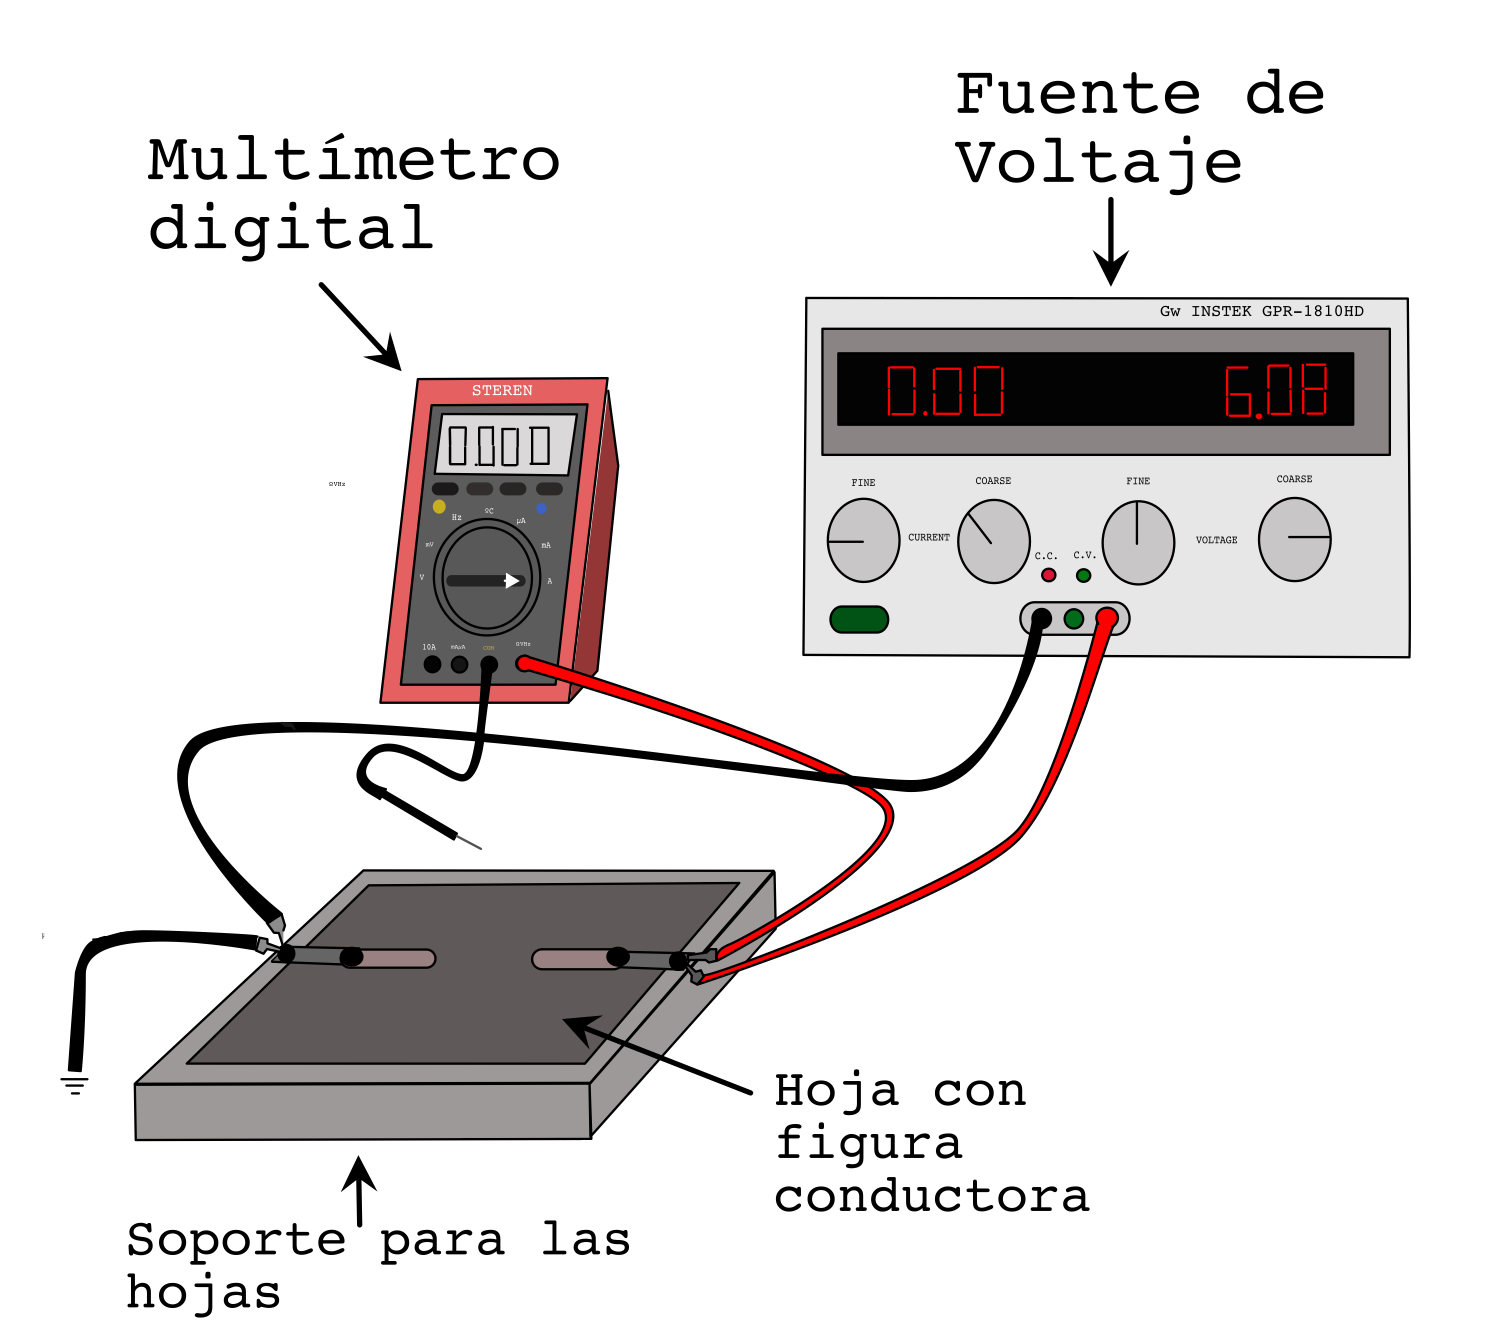
\includegraphics[scale=0.15]{soyputo2.png}
    \centering
    \caption{Diagrama del arreglo experimental}
    \label{arreglo}
\end{figure}



%%% Descripción del Montaje %%%

%COMO VERGA REFERENCIO UNA IMAGEN
Como podemos observar en la \textbf{Figura \ref{arreglo}}, la fuente de voltaje fue conectada al soporte de las hojas mediante dos especies de  pinzas que mantenían a las hojas estáticas. Estas pinzas funcionaban como un dipolo eléctrico, puesto que una de ellas fue conectada a la entrada positiva de la fuente de voltaje, mientras que la pinza contraria era conectada a la entrada negativa de la misma fuente. Asimismo, la punta de prueba conectada a la terminal $HzV\Omega$ del multímetro fue conectada de forma fija a la pinza con carga positiva, dejando libre la punta de prueba conectada a la terminal COM del multímetro, que sería la punta con la que más tarde se capturarían los datos de potencial. En el caso del arreglo de línea, la pinza conectada a la entrada negativa de la fuente de voltaje, fue adicionalmente conectada a tierra, con el fin de ver si provocaba una diferencia en los resultados. Estas pinzas, una vez colocada la hoja conductora, indujeron un polo positivo desde el cual salían las cargas, y un polo negativo a dónde iban a parar.


Fueron empleadas dos hojas con distintas figuras conductoras. La primera de ellas presentaba una figura conductora que asemejaba un dipolo básico, como se muestra en la \textbf{Figura \ref{hoja1}}, el cual simulaba un distribución continua de carga en forma de línea (\textit{arreglo de línea}). 

\begin{figure}[H]
    \centering
    \captionsetup{justification=centering,margin=0.5cm}
    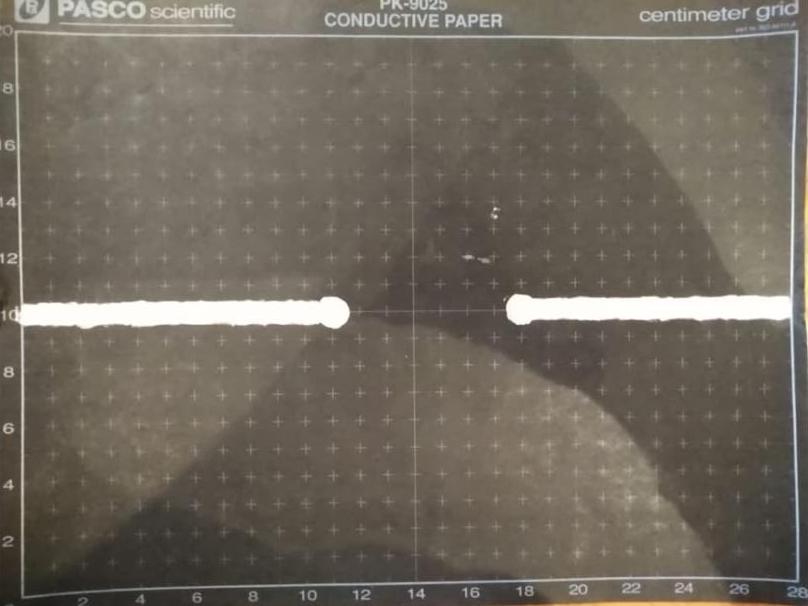
\includegraphics[scale=0.25]{wannabeyoursivonne.jpeg}
    \caption{Hoja conductora con una distribución de carga continua en forma de línea.}
    \label{hoja1}
\end{figure}

La segunda presentaba una figura conductora con forma de “T” (\textit{arreglo de placas}) en cada extremo, como se muestra en la \textbf{Figura \ref{hoja 2}}, simulando un arreglo de placas cargadas.

\begin{figure}[H]
    \centering
    \captionsetup{justification=centering,margin=0.5cm}
    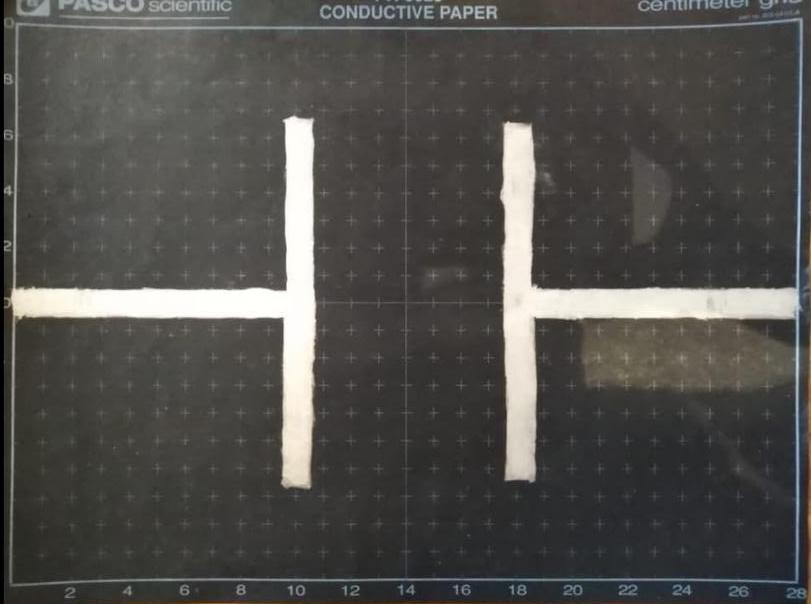
\includegraphics[scale=0.25]{andaconmigoivonne.jpeg}
    \caption{Hoja conductora con una distribución de carga continua en forma de T "placas".}
    \label{hoja 2}
\end{figure}

Empleando la punta de prueba libre del multímetro, se midió el potencial eléctrico en cada punto marcado de la hoja conductora. Fue tocándose la hoja con la punta de prueba, tal como se muestra en la \textbf{Figura \ref{med}}, y haciendo uso de Excel se diseñó una "malla", de forma que a cada celda le fue asociada una coordenada $(x, y)$ relacionada con la posición en dónde era medido el voltaje; de manera que a cada punto distinto de la hoja correspondía una celda cuyo valor era dictado por el multímetro.

\begin{figure}[H]
    \captionsetup{justification=centering,margin=0.5cm}
    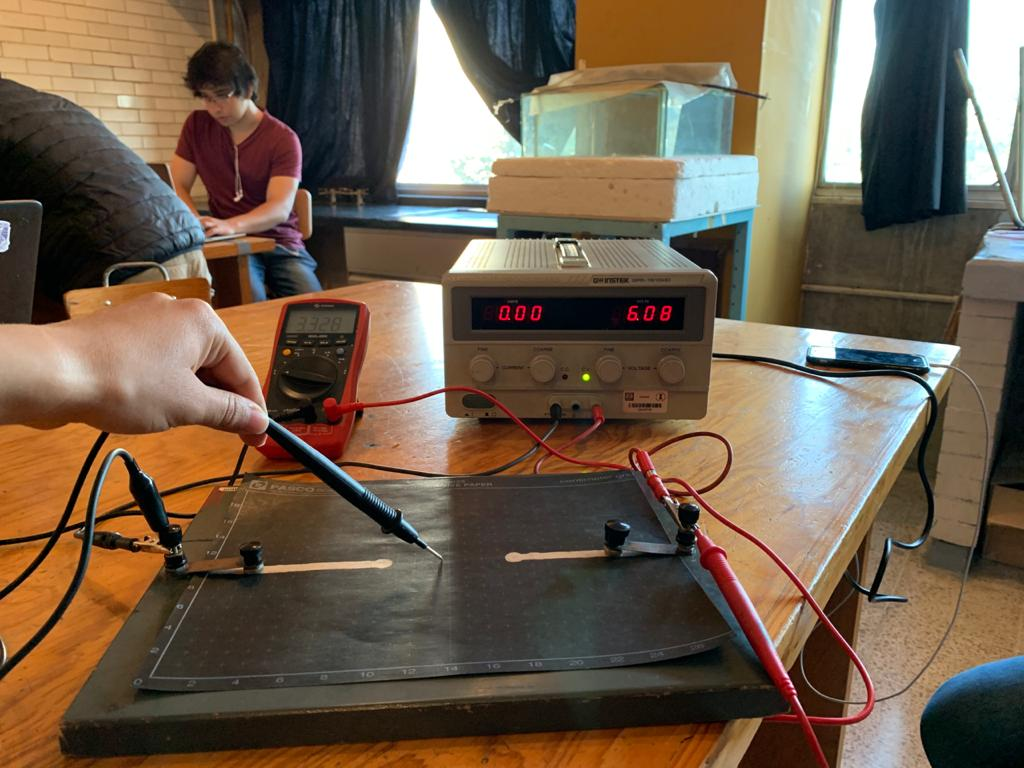
\includegraphics[scale=0.18]{putomiguel.jpeg}
    \centering
    \caption{Foto del montaje realizado, mapeo del potencial eléctrico de las coordenadas de la hoja.}
    \label{med}
\end{figure}

%%%%%%%%%

Una vez obtenidas las tablas de datos, estas se analizaron mediante el software \textit{MatLab}. Primero se realizó un análisis para asociar a cada valor de potencial un color en escala de intensidad, de forma que fuera visible su cambio y distribución sobre la hoja. Posteriormente, se trazaron las líneas equipotenciales, y mediante la relación matemática de campo y potencial dada en la \textbf{Ecuación \ref{grad}}, se determinaron los vectores de fuerza del campo eléctrico. Este último análisis, por tratarse de una función vectorial, nos arrojaría dos tablas de datos: una para las componentes en $x$ y otra para las componentes en $y$. De nuevo, mediante el análisis en \textit{MatLab}, fue posible integrar dichos datos. El código utilizado en cada sección se anexa en el \textbf{Apéndice A}.

\section{Resultados, análisis y discusión}

Los resultados se dividen en dos secciones según sea el arreglo de placas que se este analizando, así pues tenemos:

\subsection*{Arreglo de línea}

Tras medir el potencial del primer arreglo se logró obtener el esquema matricial que se muestra en la \textbf{Figura \ref{campodipolo}}.

\begin{figure}[H]
    \captionsetup{justification=centering,margin=0.5cm}
    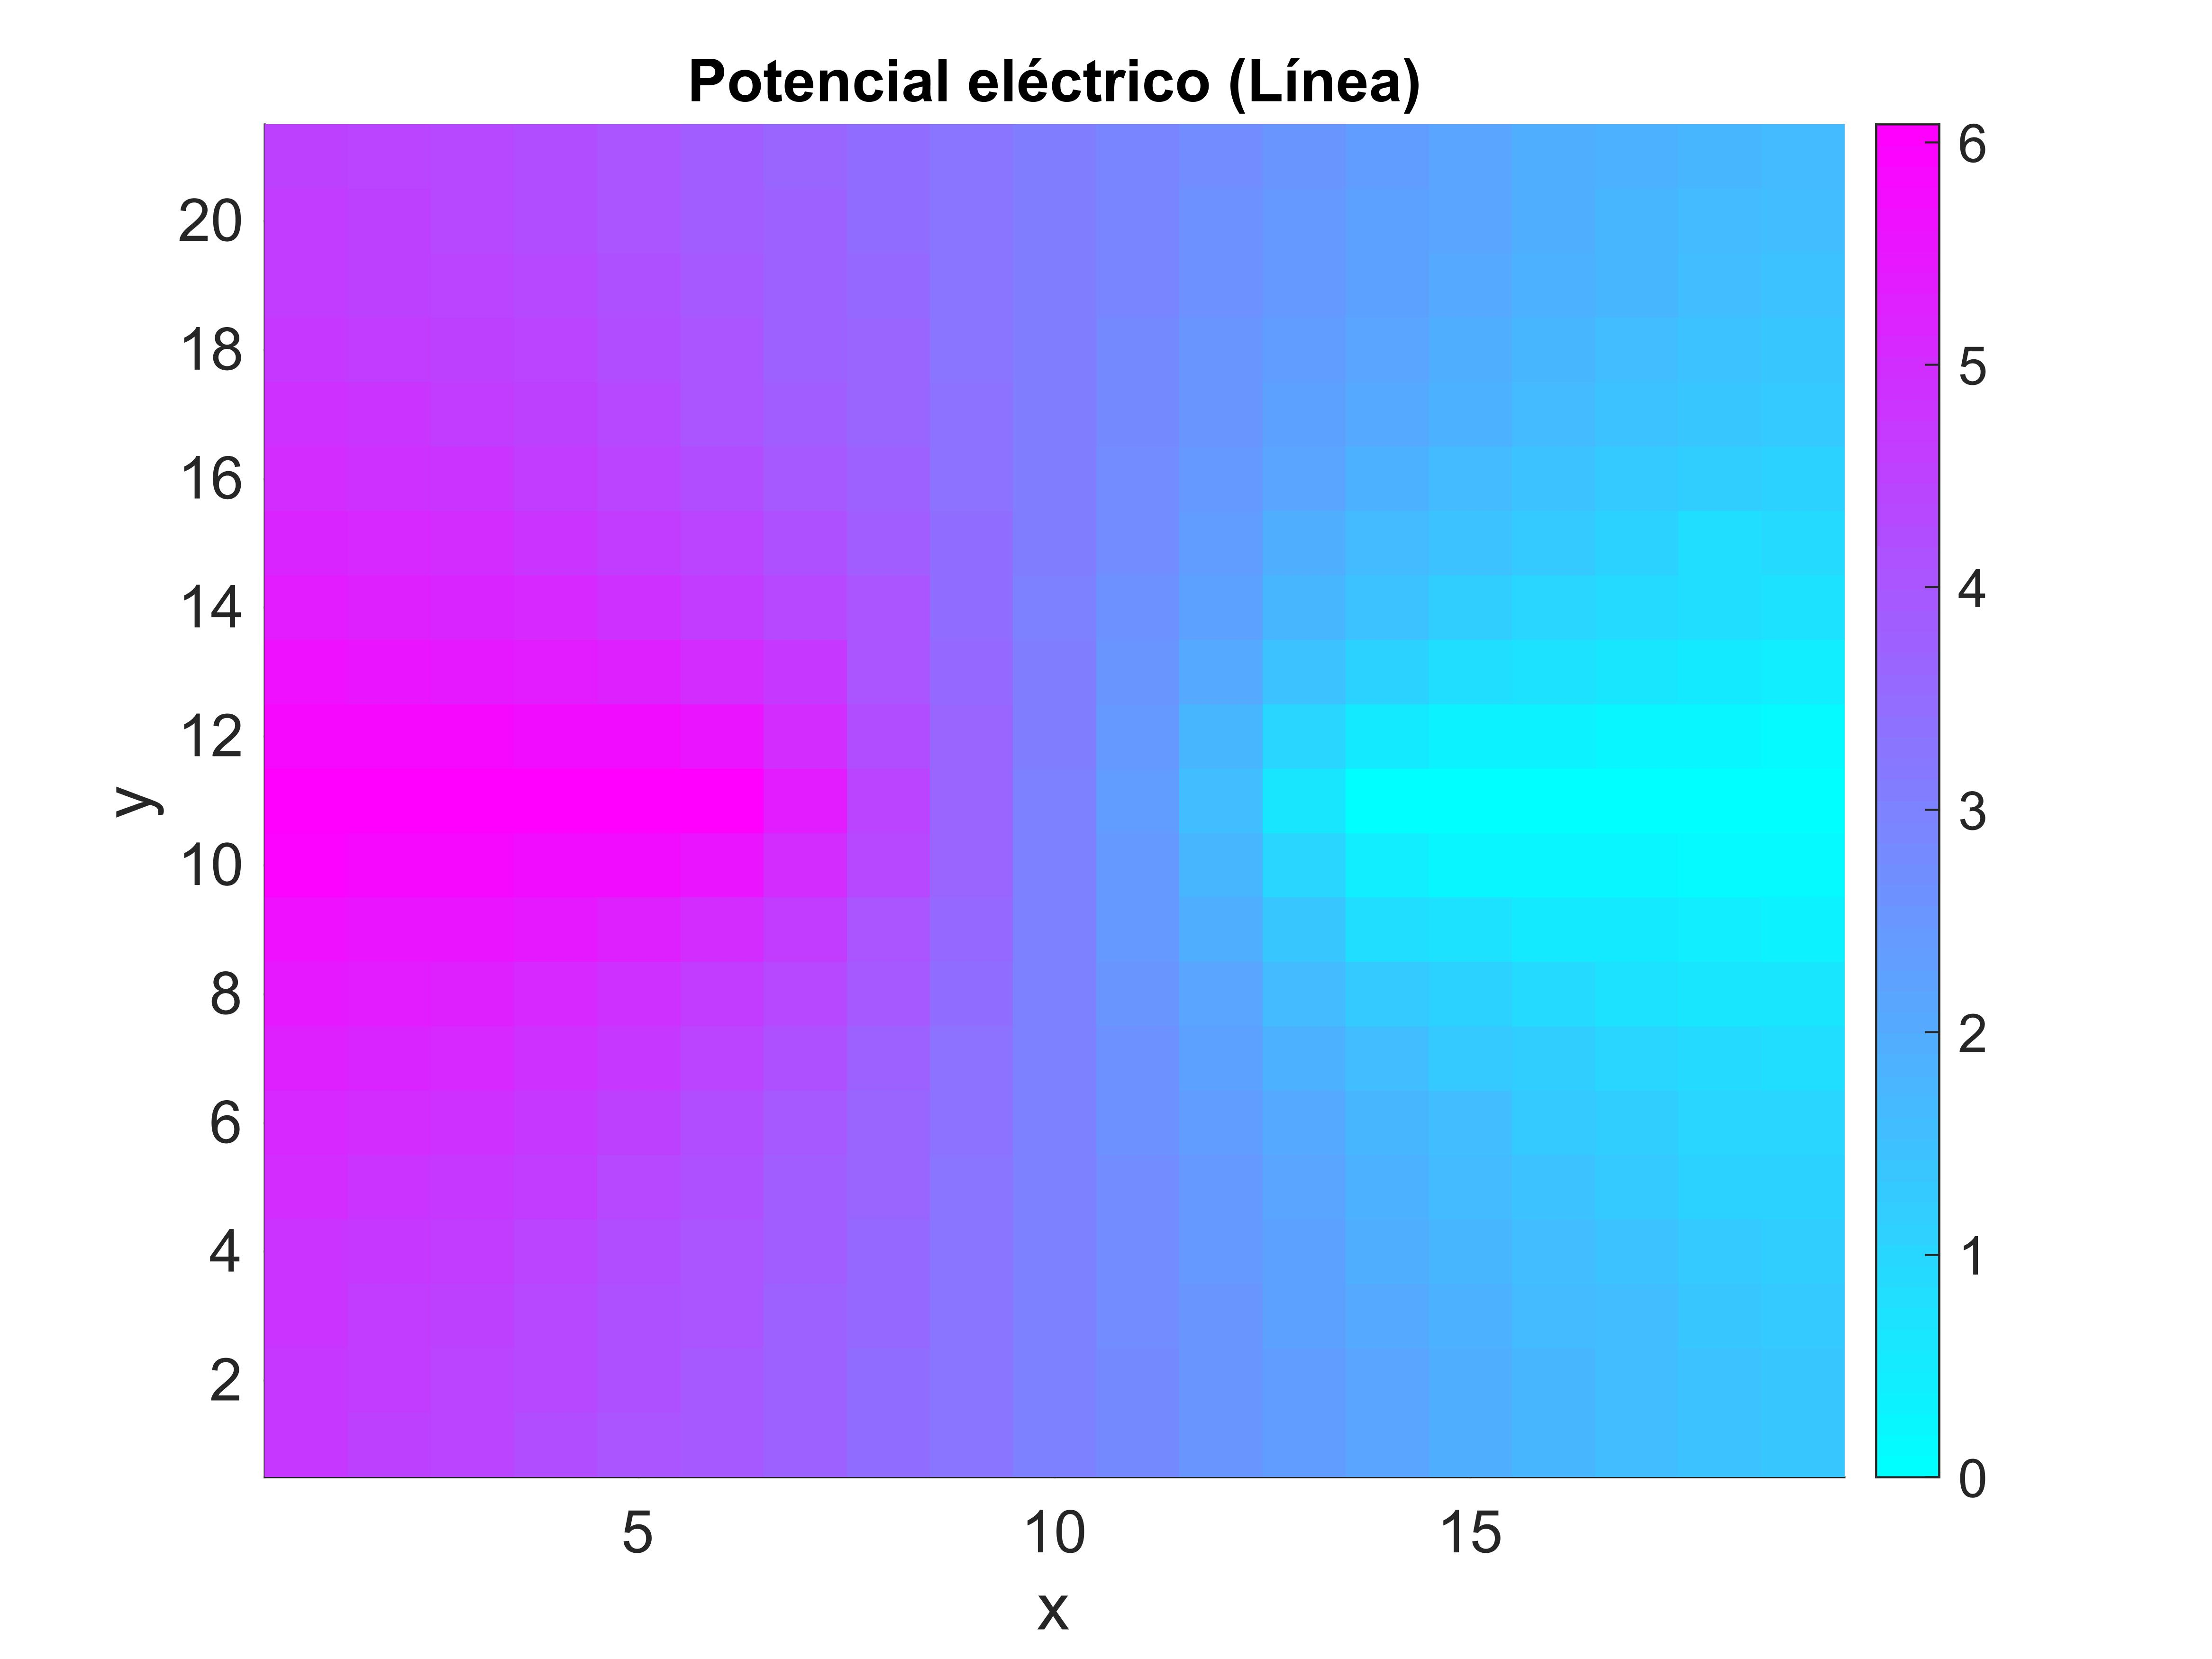
\includegraphics[scale=0.047]{dipolo.jpg}
    \centering
    \caption{Diagrama del potencial eléctrico para el sistema de línea.}
    \label{campodipolo}
\end{figure}

En el diagrama matricial se pueden observar dos secciones claramente definidas por la homogeneidad del color en sus casillas. En este caso delimitan las dos líneas que se encontraban conectadas a la fuente de voltaje, por ello una de estas líneas —color rosa— es homogénea en el valor del voltaje con el que trabajamos, es decir (6.12 $\pm$ 0.06) V, mientras que en la línea del extremo opuesto permanece constante en ceros. 

Notemos que, aunque el potencial sea cero, no significa que no se haya inducido un campo sobre el papel conductor, pues el multímetro mide una diferencia de potencial que depende de donde se haya posicionado la punta de prueba de voltaje. Como esta se colocó en la pinza positiva, la diferencia de potencial sobre toda la línea de conducción conectada a esta tendrá voltaje cero, mientras que su contraparte tendrá una diferencia de (6.12 $\pm$ 0.06) V.

Su comportamiento, sin embrago, no queda del todo claro. Por ello se realizó un segundo análisis con el fin de trazar las líneas equipotenciales, de esta forma se obtuvo la \textbf{Figura \ref{equi}}:

\begin{figure}[H]
    \captionsetup{justification=centering,margin=0.5cm}
    \centering
    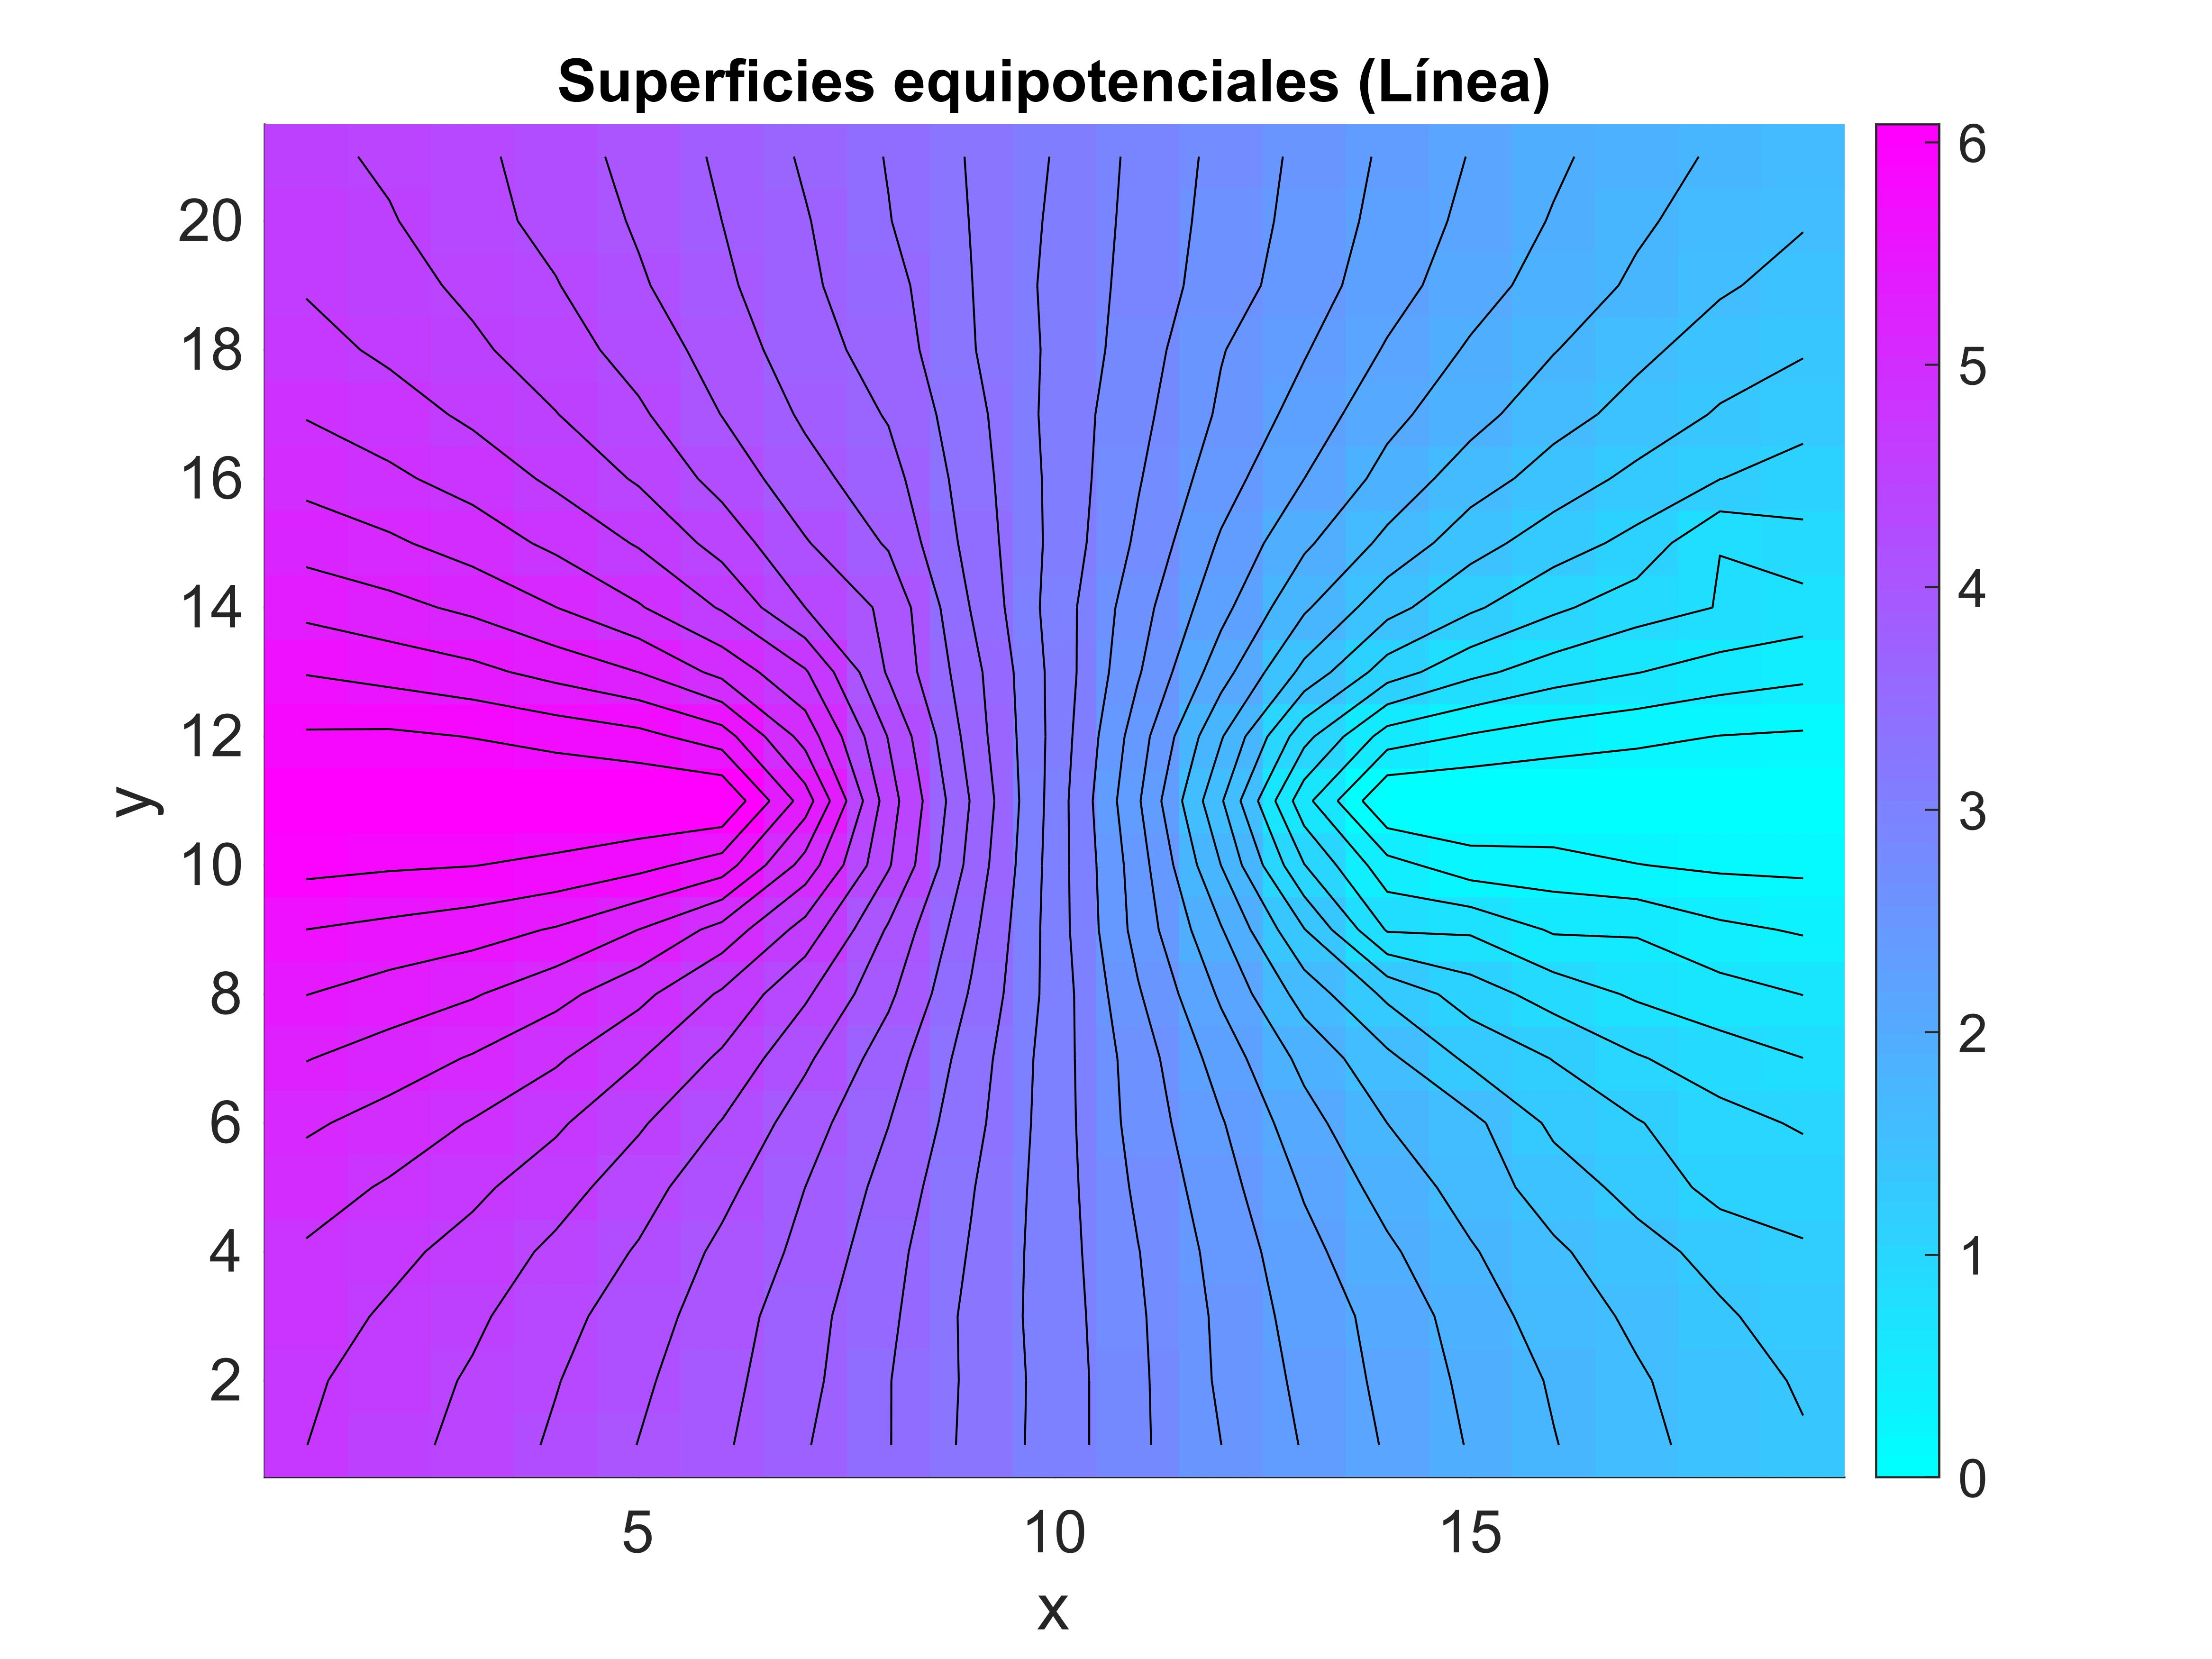
\includegraphics[scale=0.05]{equilin.jpg}
    \caption{Diagrama de las líneas equipotenciales para el arreglo de línea.}
    \label{equi}
\end{figure}

En este nuevo diagrama se logra observar mejor el comportamiento del campo eléctrico. Se puede observar que las líneas equipotenciales intentan rodear a las líneas de conducción; sin embargo, debido a la limitación espacial del sistema que tomamos en cuenta, no logramos observar este efecto por completo. También es importante mencionar que las líneas equipotenciales trazadas no son del todo uniformes debido a los errores sistemáticos que pudimos cometer al momento de la captura de datos.

Posteriormente, se obtuvieron los vectores de fuerza del campo eléctrico los cuales se observan en la \textbf{Figura \ref{camp}}.

\begin{figure}[H]
    \centering
    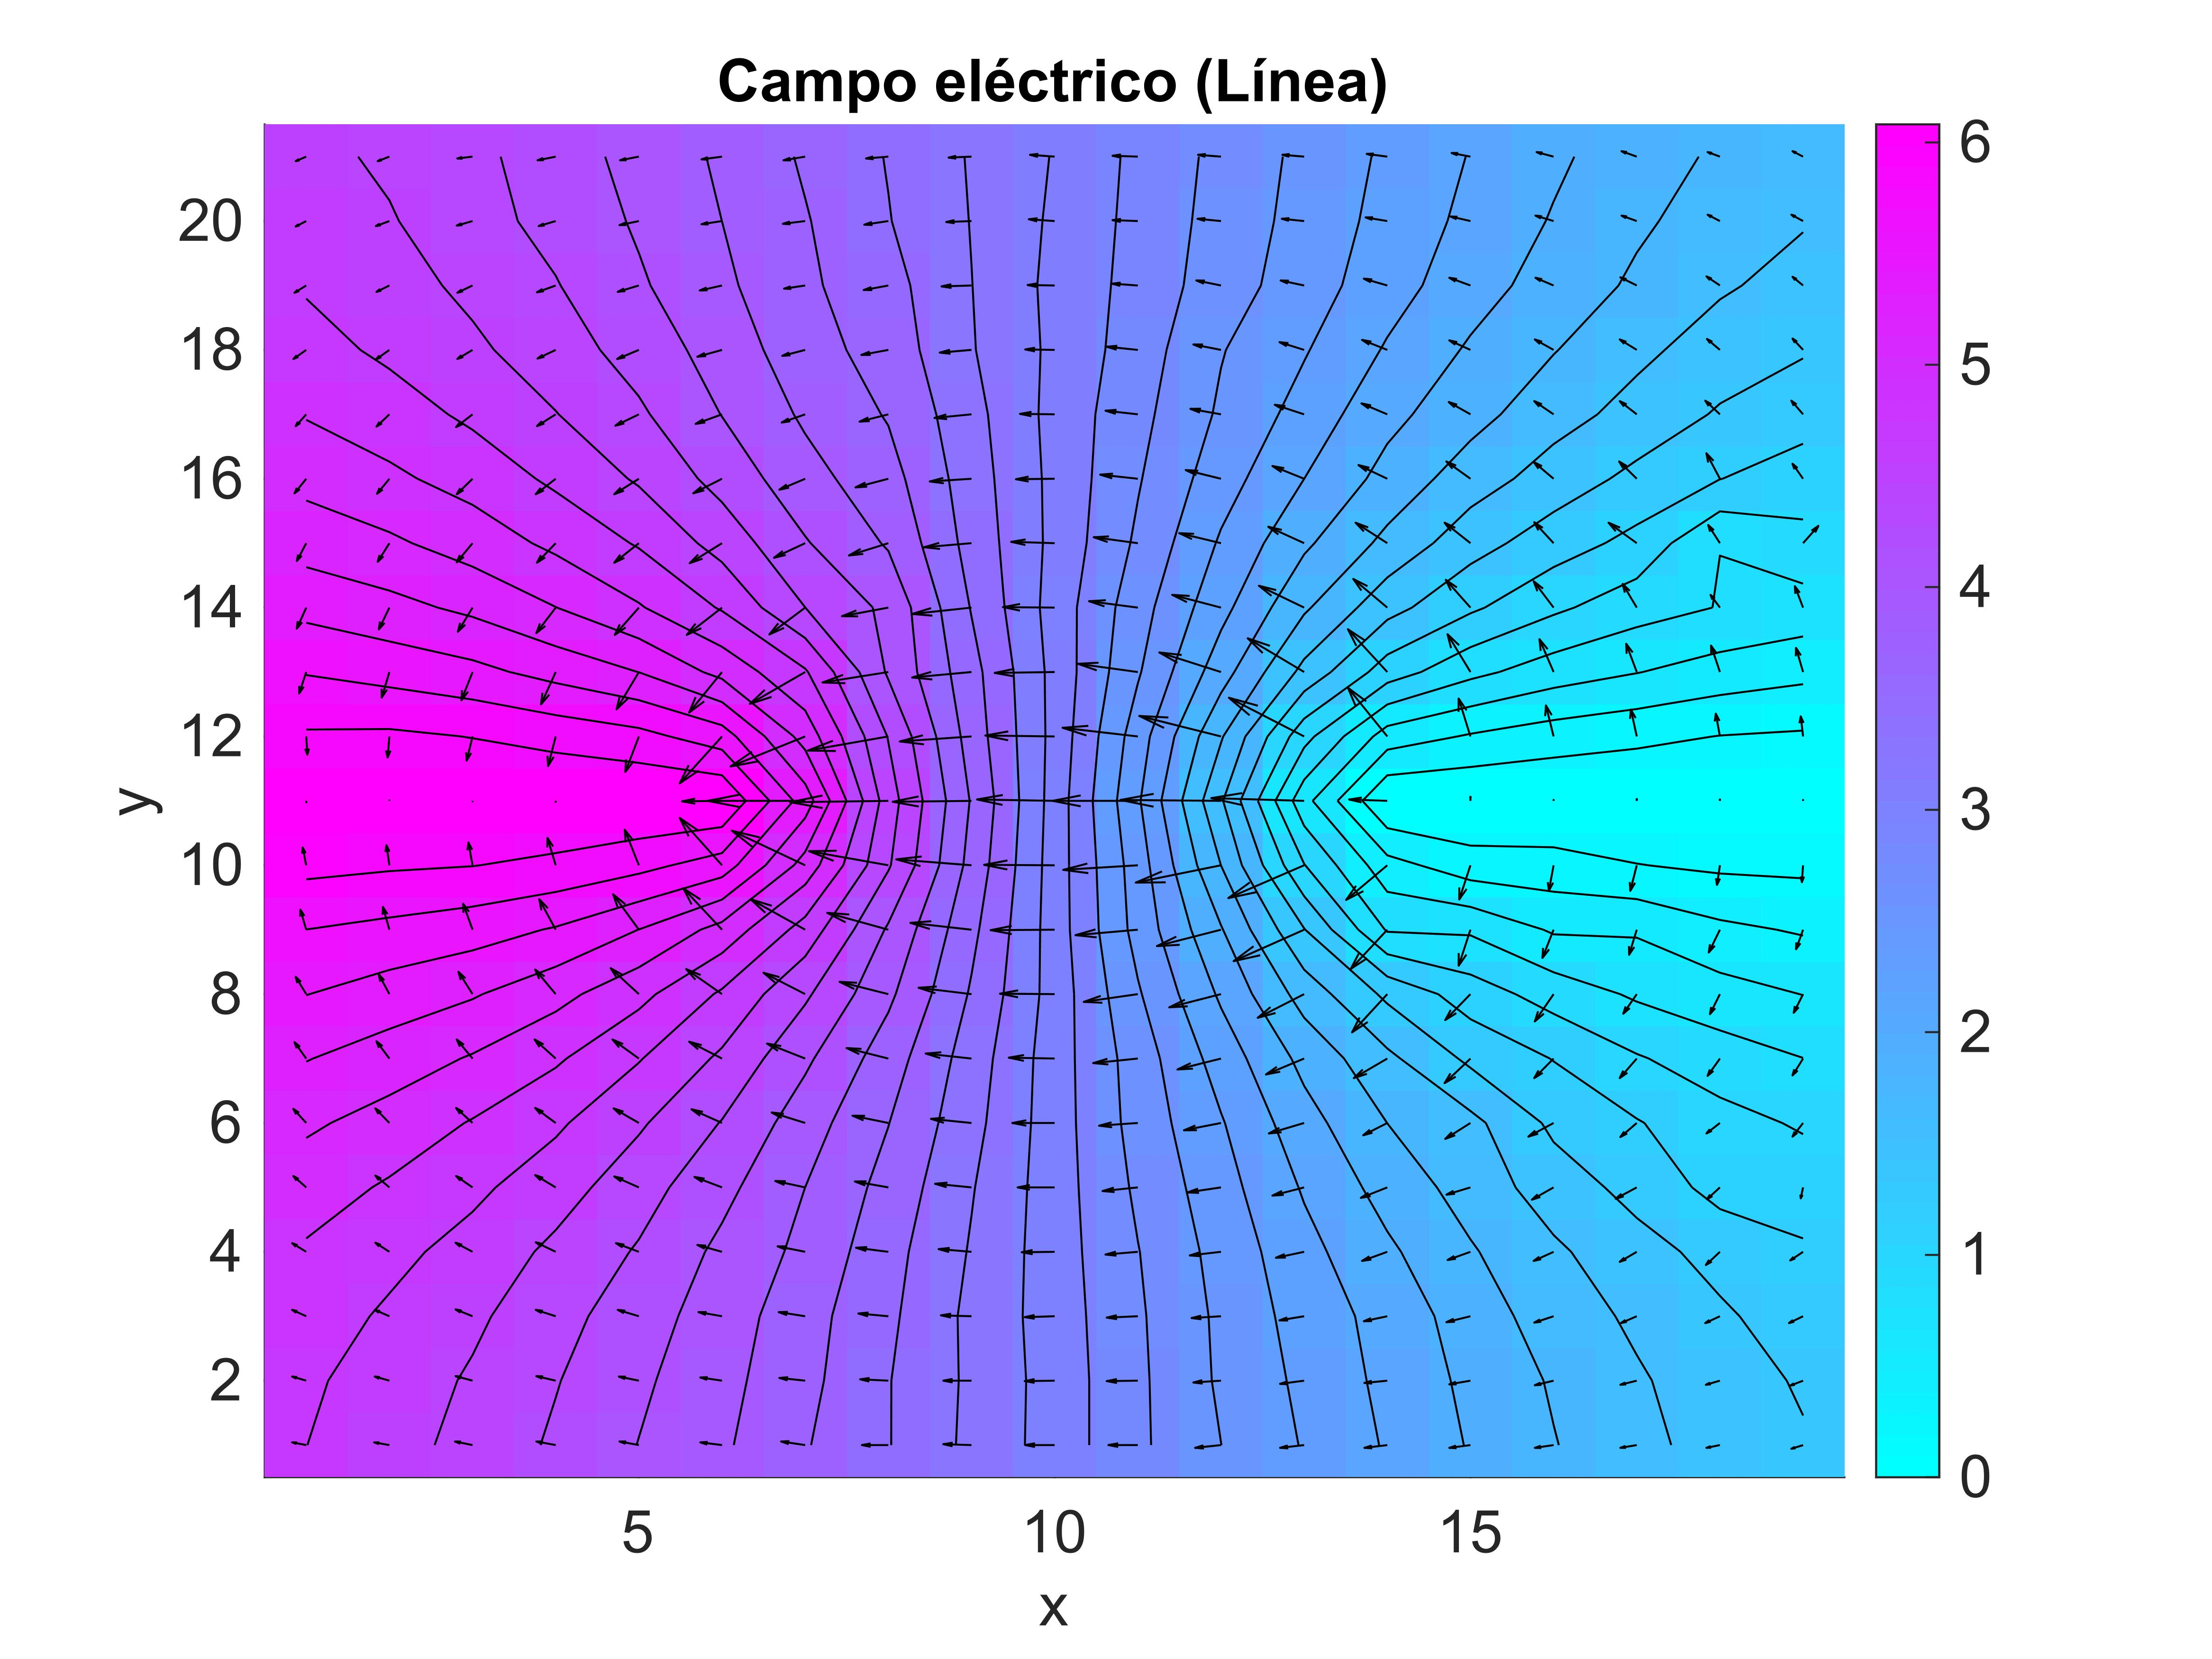
\includegraphics[scale=0.05]{finaldipolo.jpg}
    \captionsetup{justification=centering,margin=0.5cm}
    \caption{Diagrama del arreglo de línea donde se observa: potencial eléctrico, líneas equipotenciales y los vectores de fuerza del campo eléctrico.}
    \label{camp}
\end{figure}

Lo primero que resalta sobre el diagrama anterior es la dirección que tienen los vectores, ya que estos parten de la línea derecha --azul-- que tiene carga positiva, y van hasta la línea izquierda --rosa-- que se encontraba conectada a tierra y a la entrada negativa de la fuente de voltaje. Esto concuerda con la teoría, y de hecho, es posible comparar este diagrama con uno teórico basado en dos cargas puntuales opuestas (\textbf{Figura \ref{di}}). 

Debido a que no obtuvimos valores exactos de las líneas equipotenciales, nos es casi imposible obtener una relación matemática que nos garantice, tal y como dice la teoría, que las líneas de fuerza del campo son perpendiculares a las líneas equipotenciales en todo punto.


Además, se puede observar que la magnitud de los vectores del campo eléctrico disminuye conforme nos alejamos de las líneas de conducción; esto se debe a que el campo eléctrico sí depende de la distancia, por ello, entre más alejados nos encontremos de la superficie que genera el campo, este tendrá menor intensidad, lo que se ve reflejado en una disminución de su magnitud. Sin embargo, este efecto no solo se refleja en los vectores de fuerza del campo, pues las líneas equipotenciales aumentan la distancia entre ellas según se alejan de las superficies de conducción. 


\subsection*{Arreglo de placas.}

En la \textbf{Figura \ref{hoja 2}} se puede observar la hoja conductora  a analizar: un símil a dos placas paralelas. Primero se realizó el esquema matricial, el cual se muestra en la \textbf{Figura \ref{popla}}.

\begin{figure}[H]
   \centering
    \captionsetup{justification=centering,margin=0.5cm}
    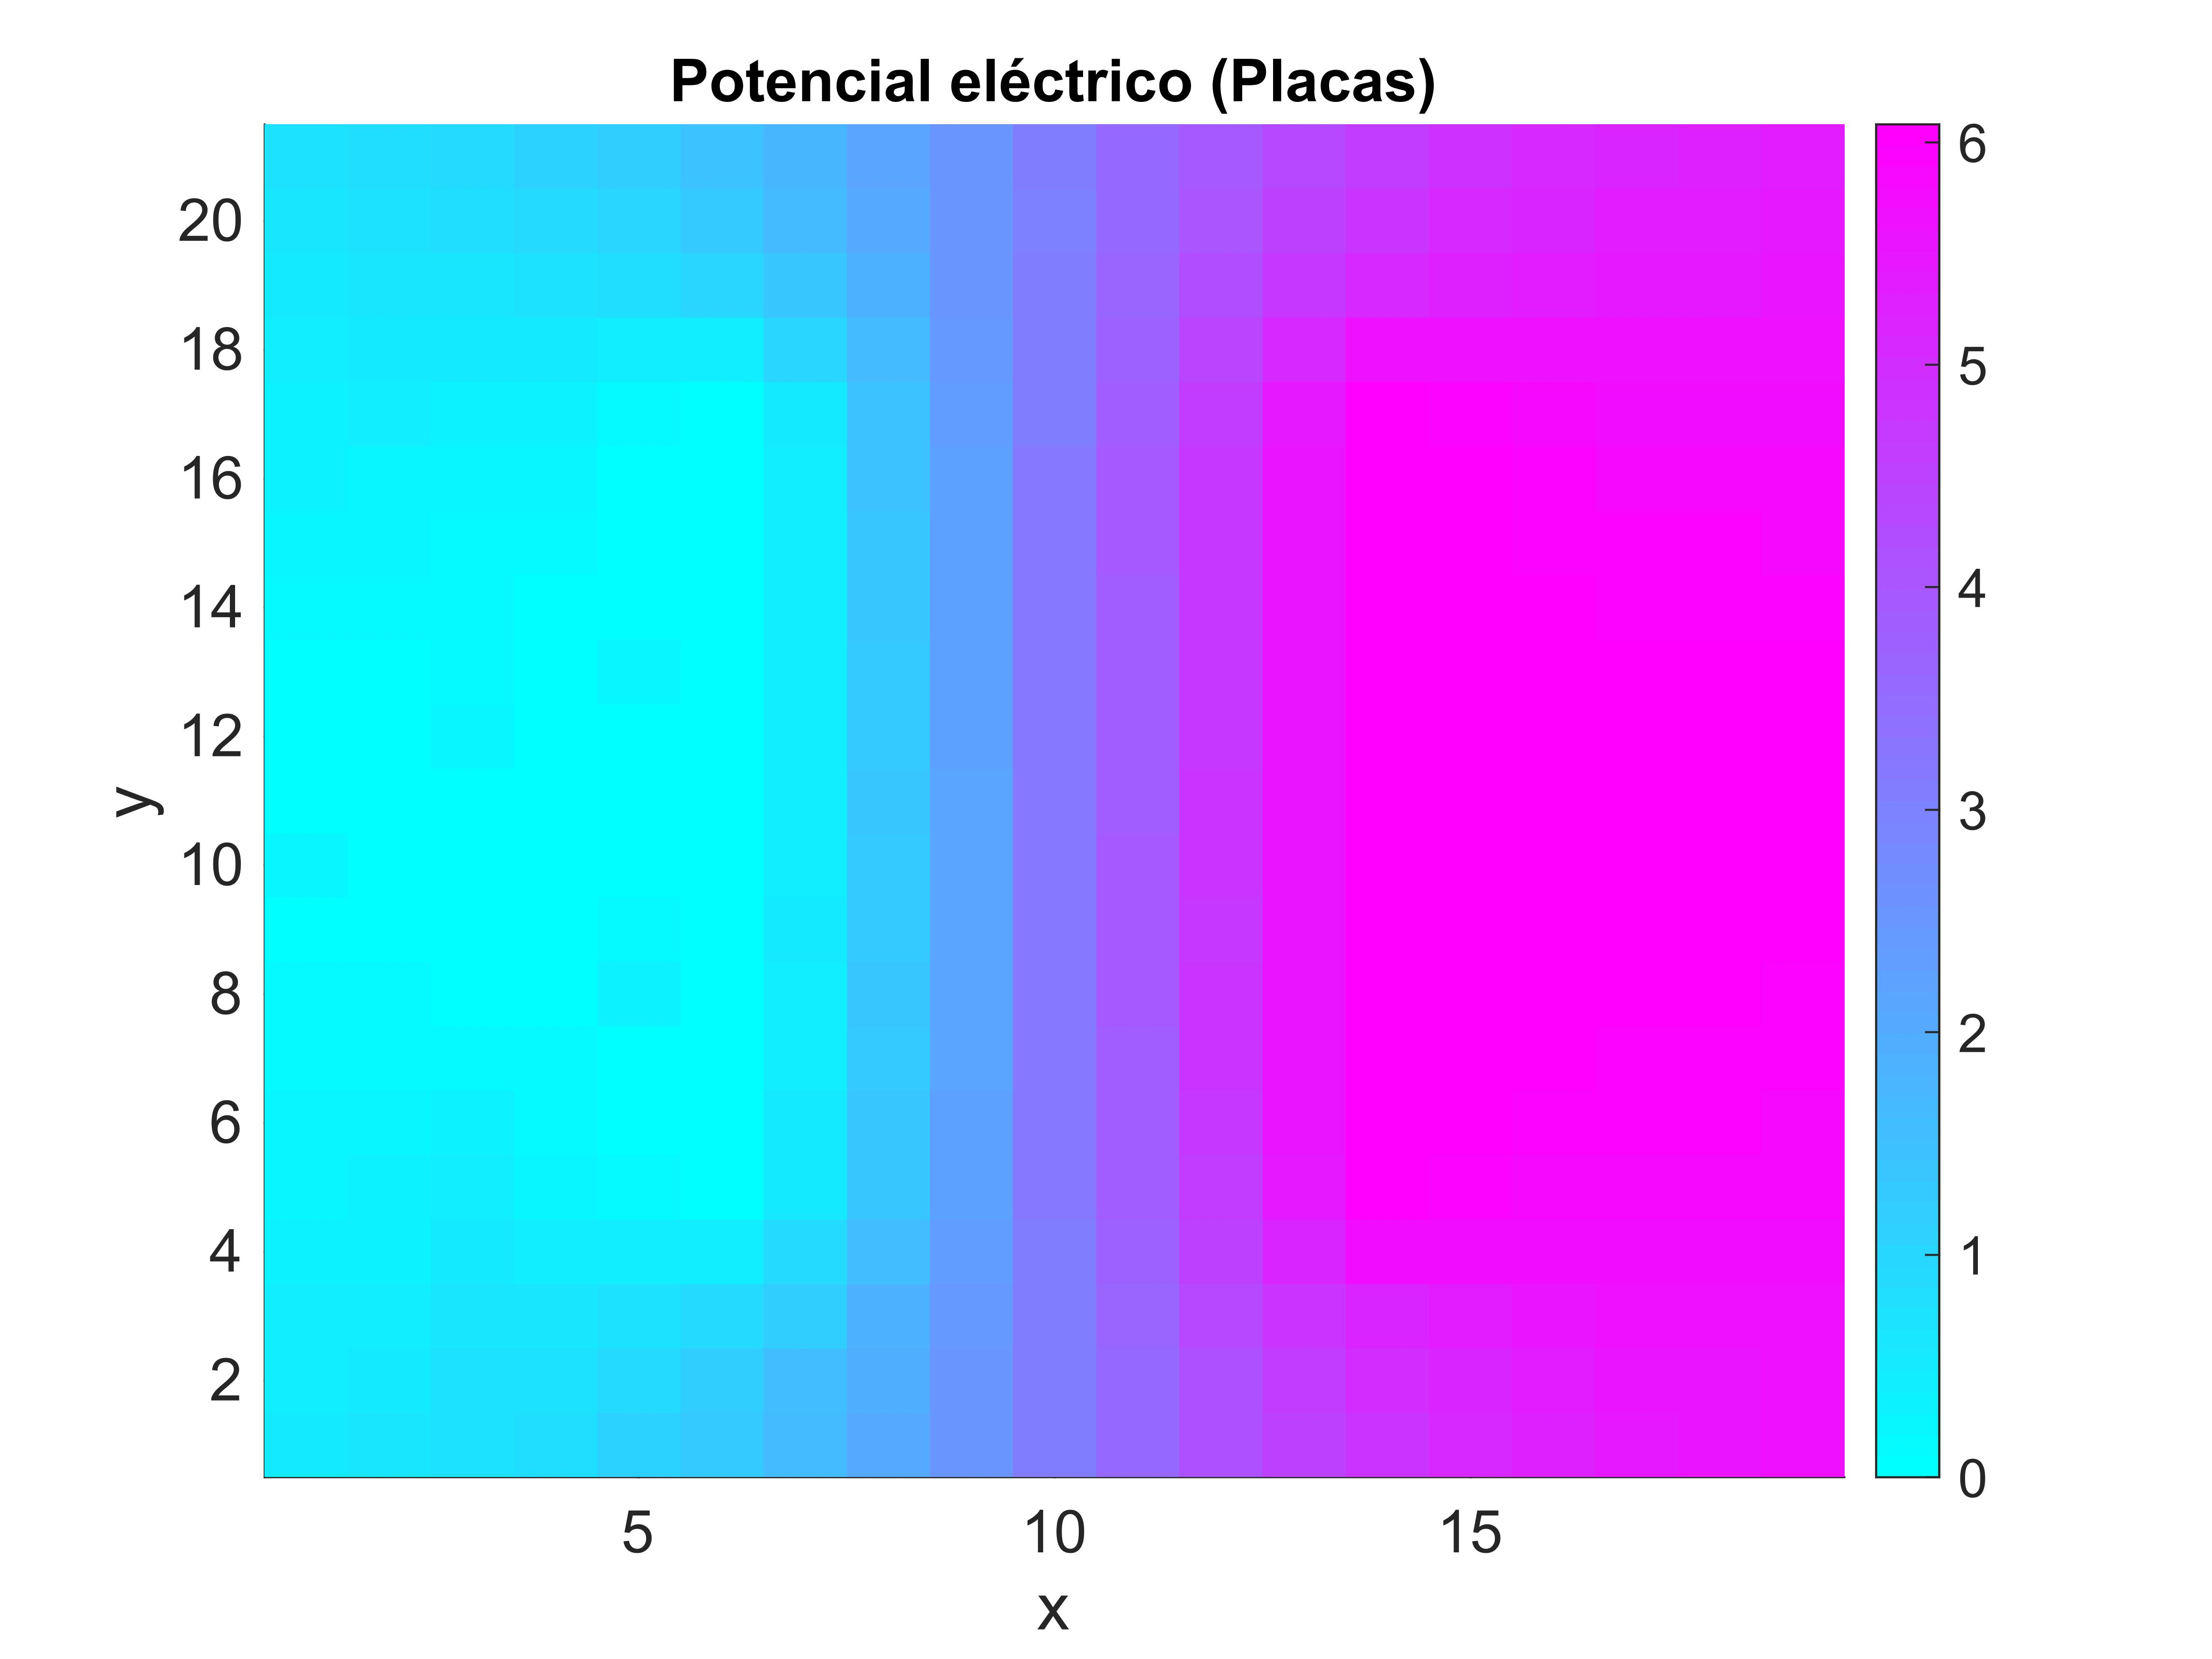
\includegraphics[scale=0.05]{placas.jpg}
    \caption{Diagrama del potencial eléctrico para el sistema de placas.}
    \label{popla}
\end{figure}

Al igual que en el arreglo anterior, hay dos regiones claramente marcadas y homogéneas en el esquema, que representan a las líneas que se encontraban conectadas a la fuente de voltaje, en este caso las placas perpendiculares. Sin embargo, estas regiones no presentan del todo la misma regularidad. Es apreciable que un par de recuadros de cada placa aumenta en potencial, que es atribuible a los errores sistemáticos que cometimos al medir.

Posteriormente, se obtuvieron las líneas equipotenciales, las cuales se muestran en \textbf{Figura \ref{equipla}}.

\begin{figure}[H]
   \centering
    \captionsetup{justification=centering,margin=0.5cm}
    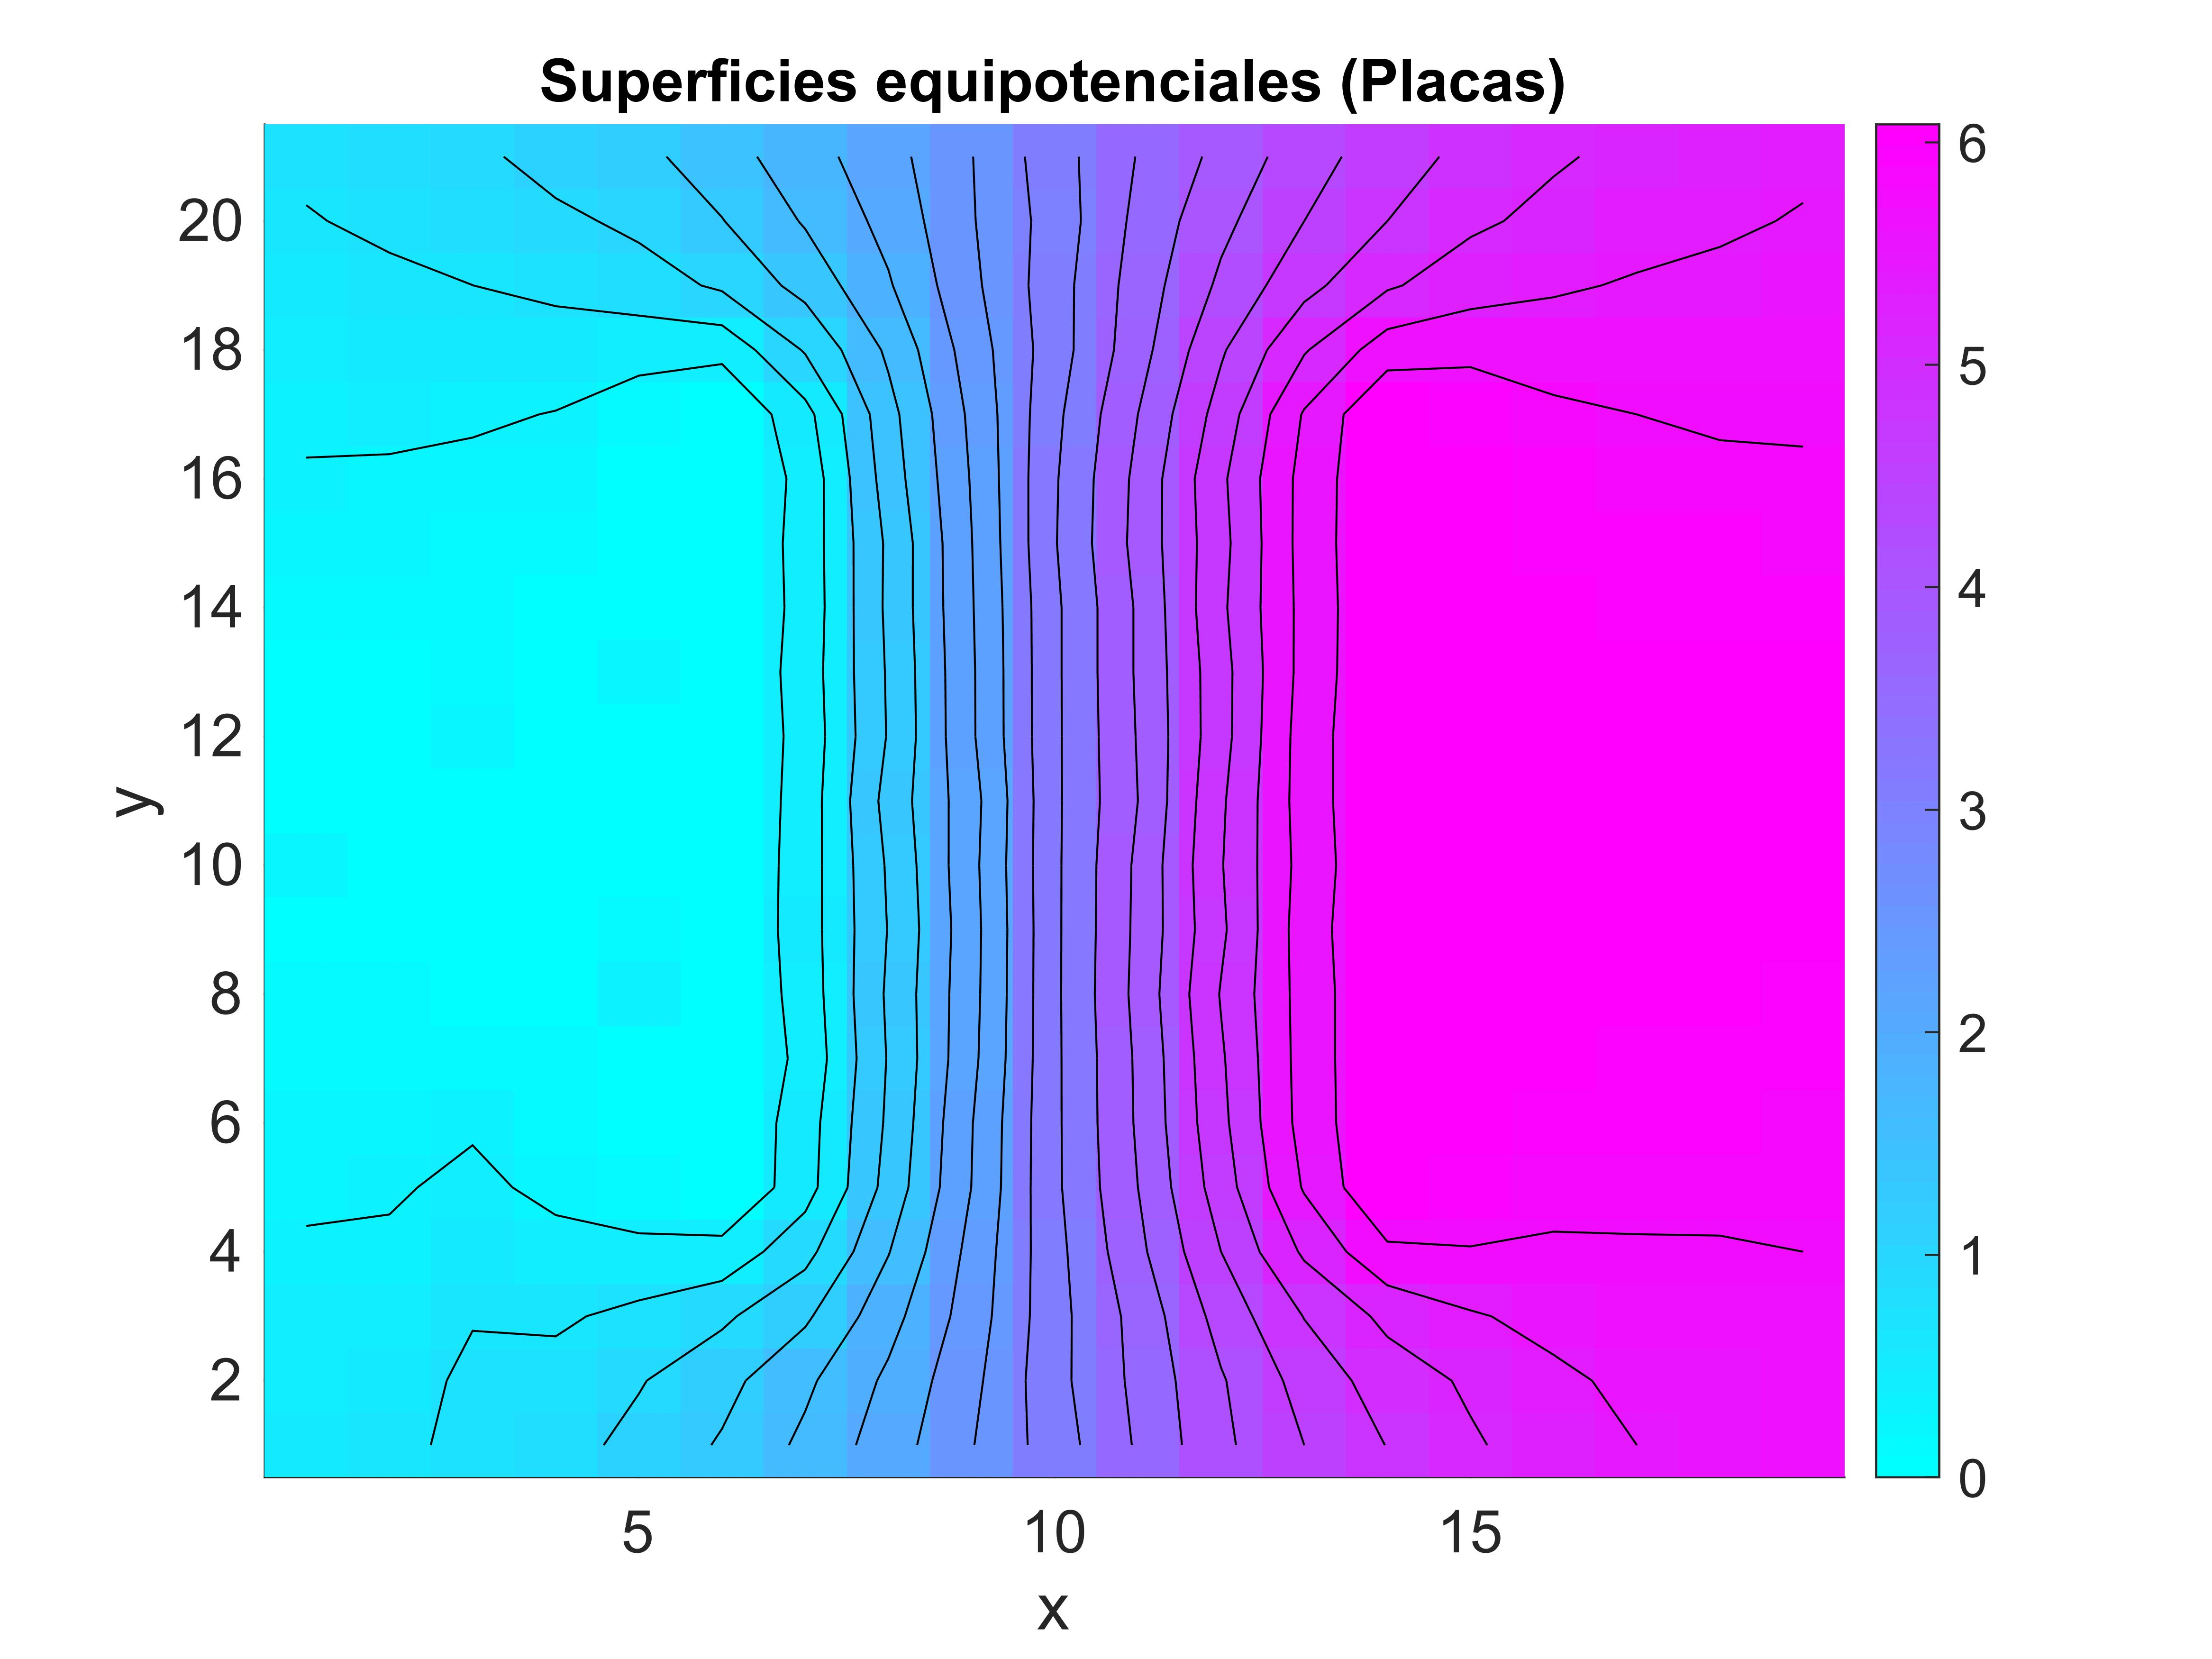
\includegraphics[scale=0.05]{equi.jpg}
    \caption{Diagrama de las líneas equipotenciales para el arreglo de placas.}
    \label{equipla}
\end{figure}

En este caso es posible observar como el potencial presenta un cambio gradual y constante entre las placas paralelas. De hecho las líneas equipotenciales permanecen paralelas a las placas, pero en cuanto se alejan de esta región, de nuevo las líneas intentan rodear las placas, similar al efecto mostrado en el arreglo anterior. Además, aquí se pueden observar mejor los errores sistemáticos que se cometieron, pues existen irregularidades más visibles en las líneas equipotenciales de la sección azul (\textbf{Figura \ref{equipla}}); dichas perturbaciones no deberían de ocurrir debido a la simetría de la hoja conductora.

Es de esperarse que, debido al comportamiento de las líneas equipotenciales, las líneas de fuerza eléctrica tengan la misma magnitud y sean perpendiculares en medio de las placas, y vuelvan a disminuir fuera de la región. Para verificar dicho comportamiento se realizó el último análisis con el fin de obtener los vectores de fuerza del campo eléctrico que se aprecia en la  \textbf{Figura \ref{finpla}} y que se muestra a continuación:

\begin{figure}[H]
	\centering
    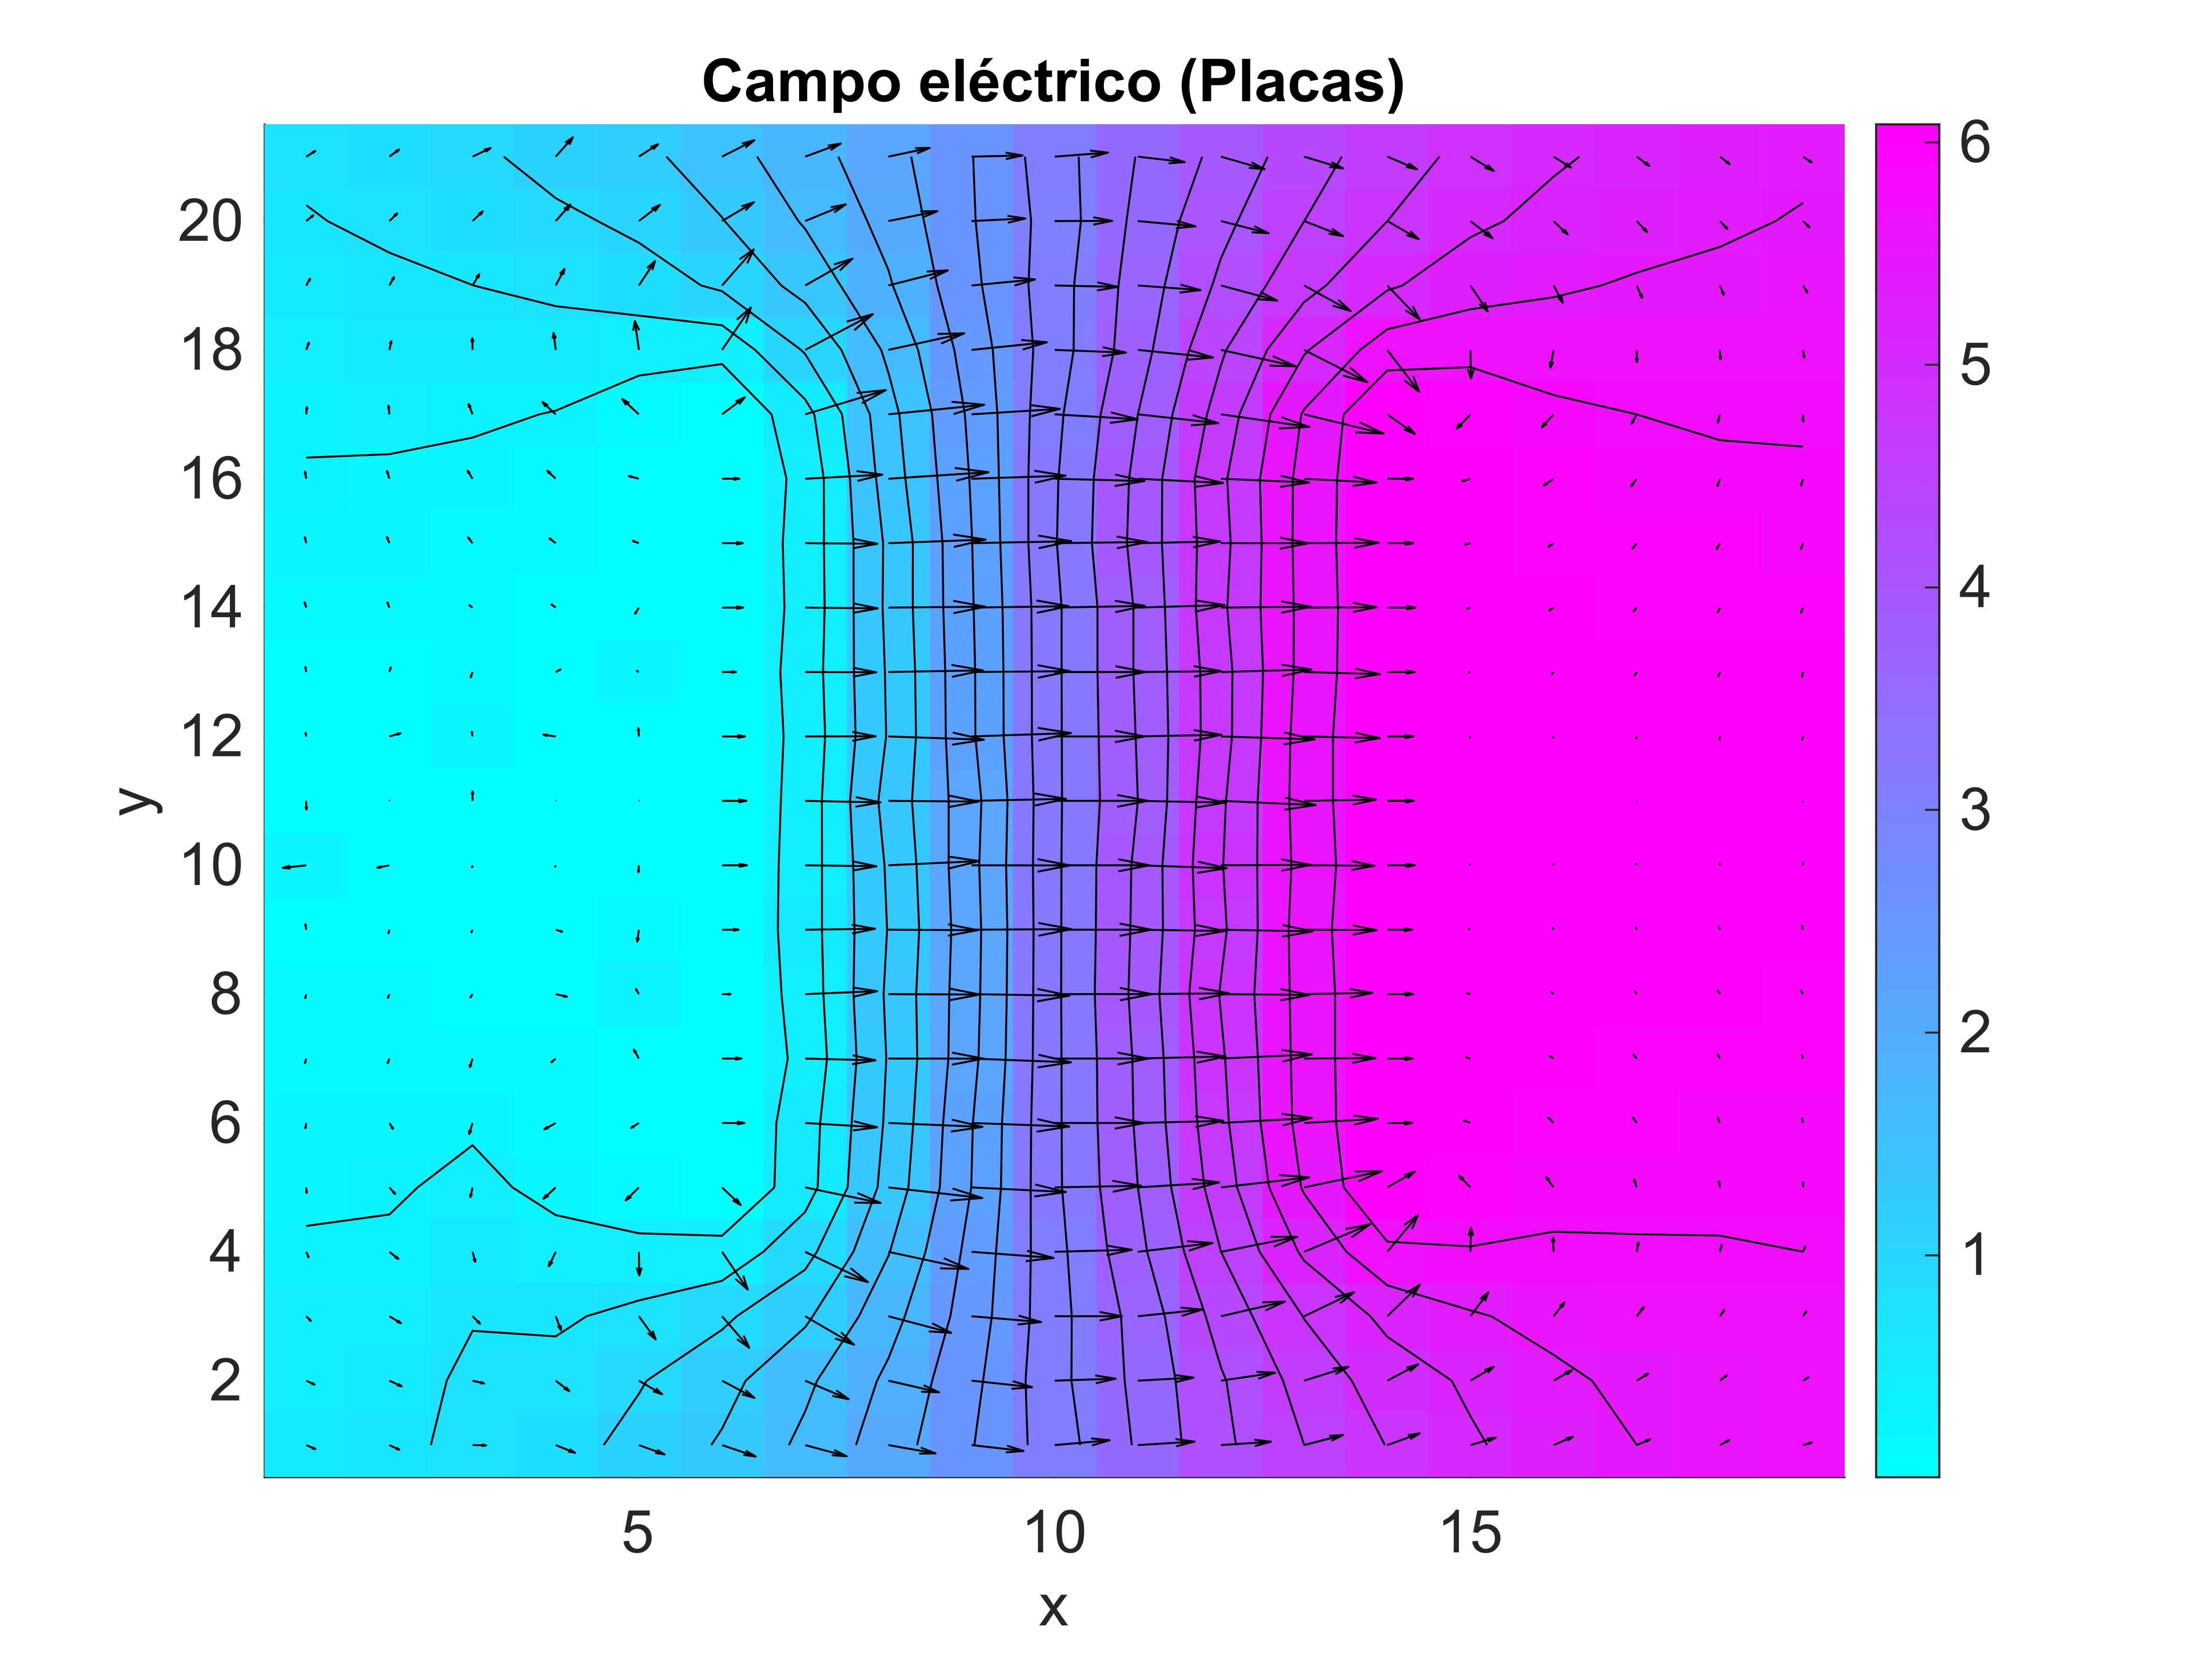
\includegraphics[scale=0.05]{finalplacas.jpg}
    \captionsetup{justification=centering,margin=0.5cm}
    \caption{Diagrama del arreglo de placas donde se observa: potencial eléctrico, líneas equipotenciales y los vectores de fuerza del campo eléctrico.}
    \label{finpla}
\end{figure}

Finalmente, observemos que, en efecto, el campo eléctrico es perpendicular a las placas, y dentro de esta región pareciera permanecer constante en magnitud; sin embargo, en cuanto sale de esta región comienza a rodear a las placas y su magnitud comienza a disminuir por la distancia que hay con respecto a las líneas que lo generan. Su dirección en la zona central indica un movimiento desde la zona azul hasta la rosa, parecido al anterior arreglo, donde los vectores van desde la placa cargada positivamente, hasta la placa que estaba conectada a tierra. Sin embargo, en este arreglo no se encontraba conectada a tierra, solo a la fuente de voltaje. Aún así, no hubo cambios significativos en las mediciones y direcciones, mas allá de las dadas por el cambio de arreglo.

La regularidad del campo entre las placas la podemos atribuir a la forma en que se distribuye el campo, es decir, para una carga puntal el campo es radial, pero en las placas tenemos una distribución uniforme de carga a lo largo de esta, por lo que entre las placas, las componentes verticales, en este caso, se anulan entre ellas, dejando únicamente la interacción de componentes horizontales.

\section{Conclusiones}

El medir el potencial eléctrico en regiones especificas de las hojas conductoras nos permitió asociar a toda una región pequeña de la hoja un valor especifico de potencial, con el fin de tener una aproximación del comportamiento del potencial en toda la hoja. Dicha aproximación, junto con ayuda del análisis computacional, nos permitió conocer las regiones donde el potencial se mantendría constante, con lo que obtuvimos las líneas equipotenciales.

Gracias a las aproximaciones obtenidas fue posible caracterizar el campo eléctrico en los dos arreglos analizados, obteniendo los valores del campo mediante las relaciones matemáticas existentes entre ambas; sin embrago, al ser datos que describían vectores, era difícil darle un sentido por si mismo, por lo que se requirió de la intervención de software que los interpretara y nos permitiera visualizar finalmente el campo eléctrico en dirección y magnitud, logrando los objetivos planteados.

Con lo anterior, podemos decir que si queremos caracterizar por completo una región de forma electrostática, podemos recurrir a medir el potencial eléctrico $V$, ya que, si conocemos el potencial, se puede obtener el campo eléctrico y viceversa; sin embargo, la facilidad de medir el potencial eléctrico y su practicidad por ser un escalar hacen más simple el caracterizar una región electrostáticamente.

Finalmente, como parte de las características que pudimos observar, fue la disminución de la intensidad del campo conforme nos alejamos de las "fuentes" que lo generan. Esto se observa mediante la separación entre si de las líneas equipotenciales y la disminución en la magnitud de los vectores de fuerza del campo. Sin embargo, no tuvimos forma de corroborar que en efecto los vectores de fuerza eran perpendiculares a las líneas equipotenciales, pues no tenemos una expresión matemática exacta que represente a las líneas equipotenciales. 

Para una mayor claridad en los resultados, además de lo referente a las líneas de campo y a las superficies equipotenciales, se recomienda medir un mayor número de coordenadas en el plano. Con esto podríamos ver un comportamiento más definido en cuanto al cambio de voltaje a través de toda la hoja; no obstante, hay que considerar el inconveniente que representa tomar tantas medidas puesto que éstas deben ser almacenadas manualmente. 


\nocite{*}
\bibliographystyle{apacite}
\bibliography{mybib}



\section*{Apéndice A: Código}

Los comandos requeridos para el análisis experimental fueron:

\begin{lstlisting}
imagesc(Potencial) \end{lstlisting} Este comando nos gráfica la distribución del potencial.
\begin{lstlisting}
contour(Potencial,40,'k') \end{lstlisting}  Este comando nos muestra la gráfica de las superficies equipotenciales, el valor 40 hace referencia a la saturación de líneas equipotenciales que se muestran.
\begin{lstlisting}
[Ex,Ey] = gradient(-Potencial) \end{lstlisting} Este comando obtiene el campo eléctrico como el gradiente negativo del potencial. Se utiliza la asignación de dos nuevos grupos de datos (Ex y Ey) con el fin de obtener coordenadas que más tarde nos permita gráficar vectores.
\begin{lstlisting}
quiver(Ex,Ey) \end{lstlisting}  Este comando nos representa los vectores del campo eléctrico de las distribuciones de cargas continua.


Finalmente se hizo una combinación de todos los comando para obtener cada una de las figuras mostradas:

Arreglo matricial del potencial eléctrico:
\begin{lstlisting}
xlabel('x'), hold on
ylabel('y')
title('Potencial electrico')
colormap('cool')
imagesc(Potencial)
\end{lstlisting}

líneas equipotenciales:
\begin{lstlisting}
xlabel('x'), hold on
ylabel('y')
title('lineas equipotenciales')
colormap('cool')
imagesc(Potencial)
contour(Potencial,30,'k')
\end{lstlisting}

Campo eléctrico:
\begin{lstlisting}
xlabel('x'), hold on
ylabel('y')
title('Campo electrico')
colormap('cool')
imagesc(Potencial)
contour(Potencial,30,'k')
quiver(Ex,Ey, 'color',[0 0 0]), hold off
\end{lstlisting}

\end{multicols}

\end{document}